\documentclass[twoside]{book}

% Packages required by doxygen
\usepackage{fixltx2e}
\usepackage{calc}
\usepackage{doxygen}
\usepackage[export]{adjustbox} % also loads graphicx
\usepackage{graphicx}
\usepackage[utf8]{inputenc}
\usepackage{makeidx}
\usepackage{multicol}
\usepackage{multirow}
\PassOptionsToPackage{warn}{textcomp}
\usepackage{textcomp}
\usepackage[nointegrals]{wasysym}
\usepackage[table]{xcolor}

% Font selection
\usepackage[T1]{fontenc}
\usepackage[scaled=.90]{helvet}
\usepackage{courier}
\usepackage{amssymb}
\usepackage{sectsty}
\renewcommand{\familydefault}{\sfdefault}
\allsectionsfont{%
  \fontseries{bc}\selectfont%
  \color{darkgray}%
}
\renewcommand{\DoxyLabelFont}{%
  \fontseries{bc}\selectfont%
  \color{darkgray}%
}
\newcommand{\+}{\discretionary{\mbox{\scriptsize$\hookleftarrow$}}{}{}}

% Page & text layout
\usepackage{geometry}
\geometry{%
  a4paper,%
  top=2.5cm,%
  bottom=2.5cm,%
  left=2.5cm,%
  right=2.5cm%
}
\tolerance=750
\hfuzz=15pt
\hbadness=750
\setlength{\emergencystretch}{15pt}
\setlength{\parindent}{0cm}
\setlength{\parskip}{0.2cm}
\makeatletter
\renewcommand{\paragraph}{%
  \@startsection{paragraph}{4}{0ex}{-1.0ex}{1.0ex}{%
    \normalfont\normalsize\bfseries\SS@parafont%
  }%
}
\renewcommand{\subparagraph}{%
  \@startsection{subparagraph}{5}{0ex}{-1.0ex}{1.0ex}{%
    \normalfont\normalsize\bfseries\SS@subparafont%
  }%
}
\makeatother

% Headers & footers
\usepackage{fancyhdr}
\pagestyle{fancyplain}
\fancyhead[LE]{\fancyplain{}{\bfseries\thepage}}
\fancyhead[CE]{\fancyplain{}{}}
\fancyhead[RE]{\fancyplain{}{\bfseries\leftmark}}
\fancyhead[LO]{\fancyplain{}{\bfseries\rightmark}}
\fancyhead[CO]{\fancyplain{}{}}
\fancyhead[RO]{\fancyplain{}{\bfseries\thepage}}
\fancyfoot[LE]{\fancyplain{}{}}
\fancyfoot[CE]{\fancyplain{}{}}
\fancyfoot[RE]{\fancyplain{}{\bfseries\scriptsize Generated on Mon Jan 4 2016 03\+:31\+:23 for Pew\+Pew by Doxygen }}
\fancyfoot[LO]{\fancyplain{}{\bfseries\scriptsize Generated on Mon Jan 4 2016 03\+:31\+:23 for Pew\+Pew by Doxygen }}
\fancyfoot[CO]{\fancyplain{}{}}
\fancyfoot[RO]{\fancyplain{}{}}
\renewcommand{\footrulewidth}{0.4pt}
\renewcommand{\chaptermark}[1]{%
  \markboth{#1}{}%
}
\renewcommand{\sectionmark}[1]{%
  \markright{\thesection\ #1}%
}

% Indices & bibliography
\usepackage{natbib}
\usepackage[titles]{tocloft}
\setcounter{tocdepth}{3}
\setcounter{secnumdepth}{5}
\makeindex

% Hyperlinks (required, but should be loaded last)
\usepackage{ifpdf}
\ifpdf
  \usepackage[pdftex,pagebackref=true]{hyperref}
\else
  \usepackage[ps2pdf,pagebackref=true]{hyperref}
\fi
\hypersetup{%
  colorlinks=true,%
  linkcolor=blue,%
  citecolor=blue,%
  unicode%
}

% Custom commands
\newcommand{\clearemptydoublepage}{%
  \newpage{\pagestyle{empty}\cleardoublepage}%
}


%===== C O N T E N T S =====

\begin{document}

% Titlepage & ToC
\hypersetup{pageanchor=false,
             bookmarks=true,
             bookmarksnumbered=true,
             pdfencoding=unicode
            }
\pagenumbering{roman}
\begin{titlepage}
\vspace*{7cm}
\begin{center}%
{\Large Pew\+Pew }\\
\vspace*{1cm}
{\large Generated by Doxygen 1.8.10}\\
\vspace*{0.5cm}
{\small Mon Jan 4 2016 03:31:23}\\
\end{center}
\end{titlepage}
\clearemptydoublepage
\tableofcontents
\clearemptydoublepage
\pagenumbering{arabic}
\hypersetup{pageanchor=true}

%--- Begin generated contents ---
\chapter{Module Index}
\section{Modules}
Here is a list of all modules\+:\begin{DoxyCompactList}
\item \contentsline{section}{game}{\pageref{group__game}}{}
\item \contentsline{section}{kbd}{\pageref{group__kbd}}{}
\item \contentsline{section}{lmlib}{\pageref{group__lmlib}}{}
\item \contentsline{section}{mouse}{\pageref{group__mouse}}{}
\item \contentsline{section}{sprite}{\pageref{group__sprite}}{}
\item \contentsline{section}{timer}{\pageref{group__timer}}{}
\item \contentsline{section}{vbe}{\pageref{group__vbe}}{}
\item \contentsline{section}{vector}{\pageref{group__vector}}{}
\item \contentsline{section}{video\+\_\+gr}{\pageref{group__video__gr}}{}
\item \contentsline{section}{xpm}{\pageref{group__xpm}}{}
\end{DoxyCompactList}

\chapter{Data Structure Index}
\section{Data Structures}
Here are the data structures with brief descriptions\+:\begin{DoxyCompactList}
\item\contentsline{section}{\hyperlink{struct____attribute____}{\+\_\+\+\_\+attribute\+\_\+\+\_\+} }{\pageref{struct____attribute____}}{}
\item\contentsline{section}{\hyperlink{structmmap__t}{mmap\+\_\+t} }{\pageref{structmmap__t}}{}
\item\contentsline{section}{\hyperlink{struct_sprite}{Sprite} }{\pageref{struct_sprite}}{}
\item\contentsline{section}{\hyperlink{structvector}{vector} }{\pageref{structvector}}{}
\end{DoxyCompactList}

\chapter{Module Documentation}
\hypertarget{group__game}{}\section{game}
\label{group__game}\index{game@{game}}
\subsection*{Functions}
\begin{DoxyCompactItemize}
\item 
int \hyperlink{group__game_ga860a3ff149bb616ec2242dc34bb52b51}{game} (char $\ast$video\+\_\+mem, int player, int time\+\_\+other\+\_\+player)
\begin{DoxyCompactList}\small\item\em Primary game function. \end{DoxyCompactList}\item 
int \hyperlink{group__game_ga792d3a7c31488479811f72b787f85e4d}{menu} (char $\ast$video\+\_\+mem)
\begin{DoxyCompactList}\small\item\em Function for displaying the menu. \end{DoxyCompactList}\item 
void \hyperlink{group__game_ga8273bb9d5ec414429bd897d7c95a1303}{player\+\_\+wins} (char $\ast$video\+\_\+mem, int player)
\begin{DoxyCompactList}\small\item\em Function for displaying the winner of the game. \end{DoxyCompactList}\end{DoxyCompactItemize}


\subsection{Detailed Description}
Functions related to game and user interface. 

\subsection{Function Documentation}
\hypertarget{group__game_ga860a3ff149bb616ec2242dc34bb52b51}{}\index{game@{game}!game@{game}}
\index{game@{game}!game@{game}}
\subsubsection[{game(char $\ast$video\+\_\+mem, int player, int time\+\_\+other\+\_\+player)}]{\setlength{\rightskip}{0pt plus 5cm}int game (
\begin{DoxyParamCaption}
\item[{char $\ast$}]{video\+\_\+mem, }
\item[{int}]{player, }
\item[{int}]{time\+\_\+other\+\_\+player}
\end{DoxyParamCaption}
)}\label{group__game_ga860a3ff149bb616ec2242dc34bb52b51}


Primary game function. 

Responsible for a player\textquotesingle{}s turn. After a turn starts it lasts until who player who is running away loses all its health.


\begin{DoxyParams}{Parameters}
{\em video\+\_\+mem} & virtual address V\+R\+A\+M was mapped to. \\
\hline
{\em player} & number of the player that will shoot this turn. \\
\hline
{\em time\+\_\+other\+\_\+player} & time the other player took completing his turn (in ms). If no other player as completed a turn this parameter should be -\/1. \\
\hline
\end{DoxyParams}
\begin{DoxyReturn}{Returns}
number of seconds the turn took. -\/1 if the the E\+S\+C key was pressed. 
\end{DoxyReturn}


Here is the call graph for this function\+:\nopagebreak
\begin{figure}[H]
\begin{center}
\leavevmode
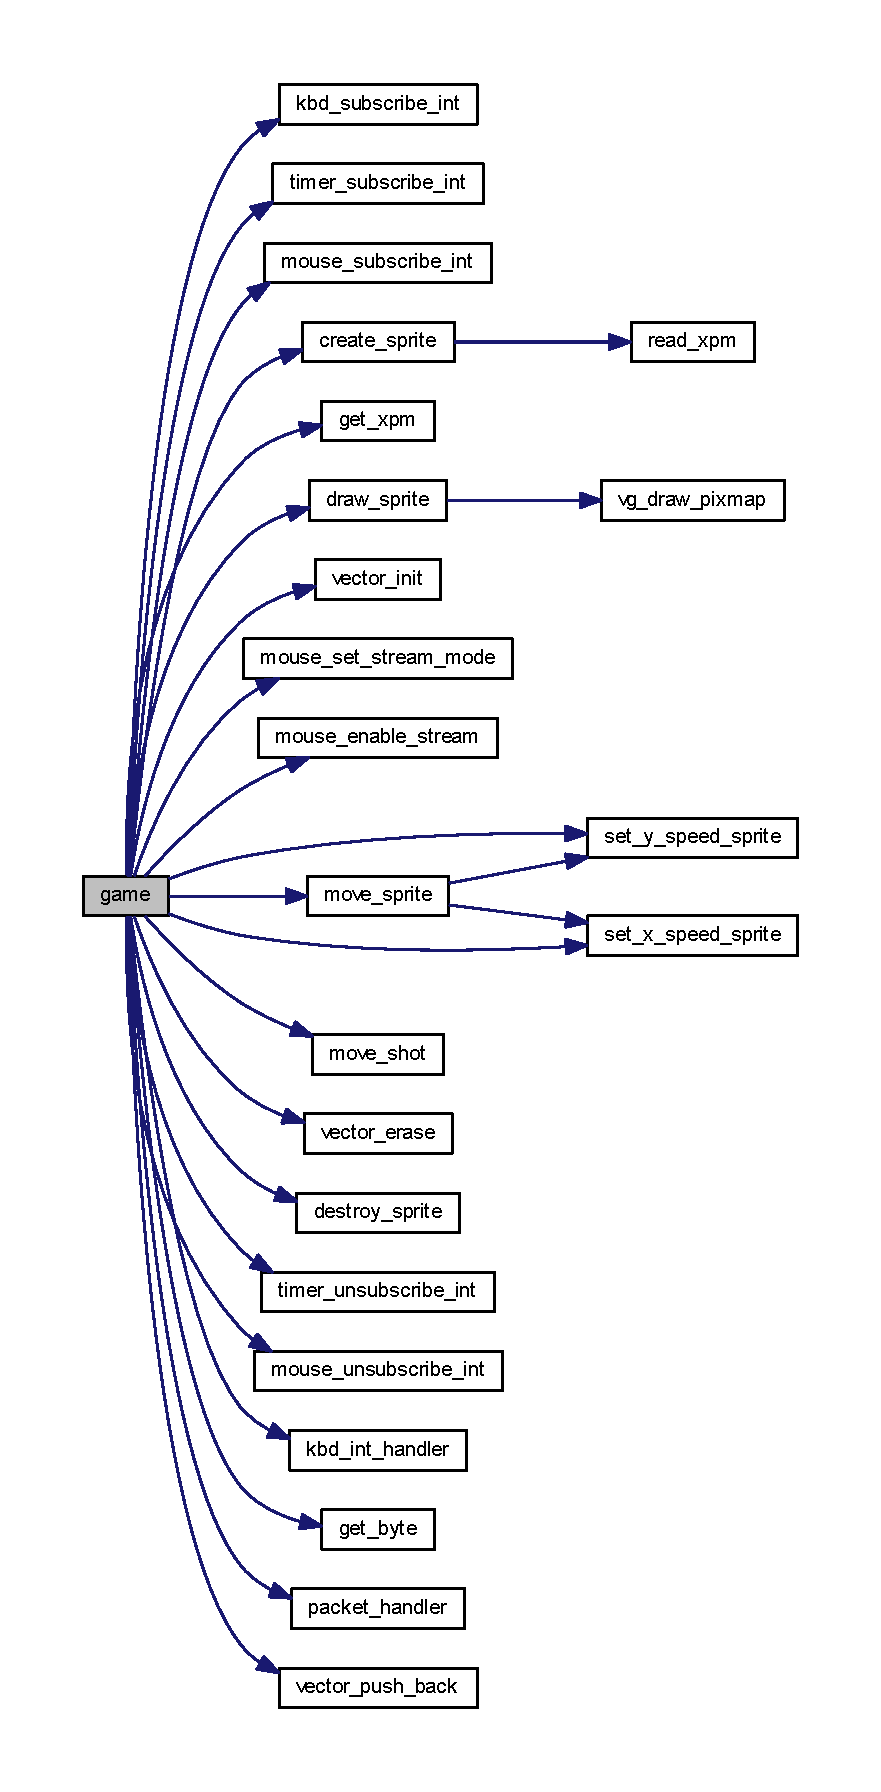
\includegraphics[height=550pt]{group__game_ga860a3ff149bb616ec2242dc34bb52b51_cgraph}
\end{center}
\end{figure}


\hypertarget{group__game_ga792d3a7c31488479811f72b787f85e4d}{}\index{game@{game}!menu@{menu}}
\index{menu@{menu}!game@{game}}
\subsubsection[{menu(char $\ast$video\+\_\+mem)}]{\setlength{\rightskip}{0pt plus 5cm}int menu (
\begin{DoxyParamCaption}
\item[{char $\ast$}]{video\+\_\+mem}
\end{DoxyParamCaption}
)}\label{group__game_ga792d3a7c31488479811f72b787f85e4d}


Function for displaying the menu. 

Responsible for displaying the menu screen and either indicate the beginning of the game or exit of the program.


\begin{DoxyParams}{Parameters}
{\em video\+\_\+mem} & virtual address V\+R\+A\+M was mapped to. \\
\hline
\end{DoxyParams}
\begin{DoxyReturn}{Returns}
0 if the user chose to begin the game. -\/1 if the E\+S\+C key was pressed. 
\end{DoxyReturn}


Here is the call graph for this function\+:\nopagebreak
\begin{figure}[H]
\begin{center}
\leavevmode
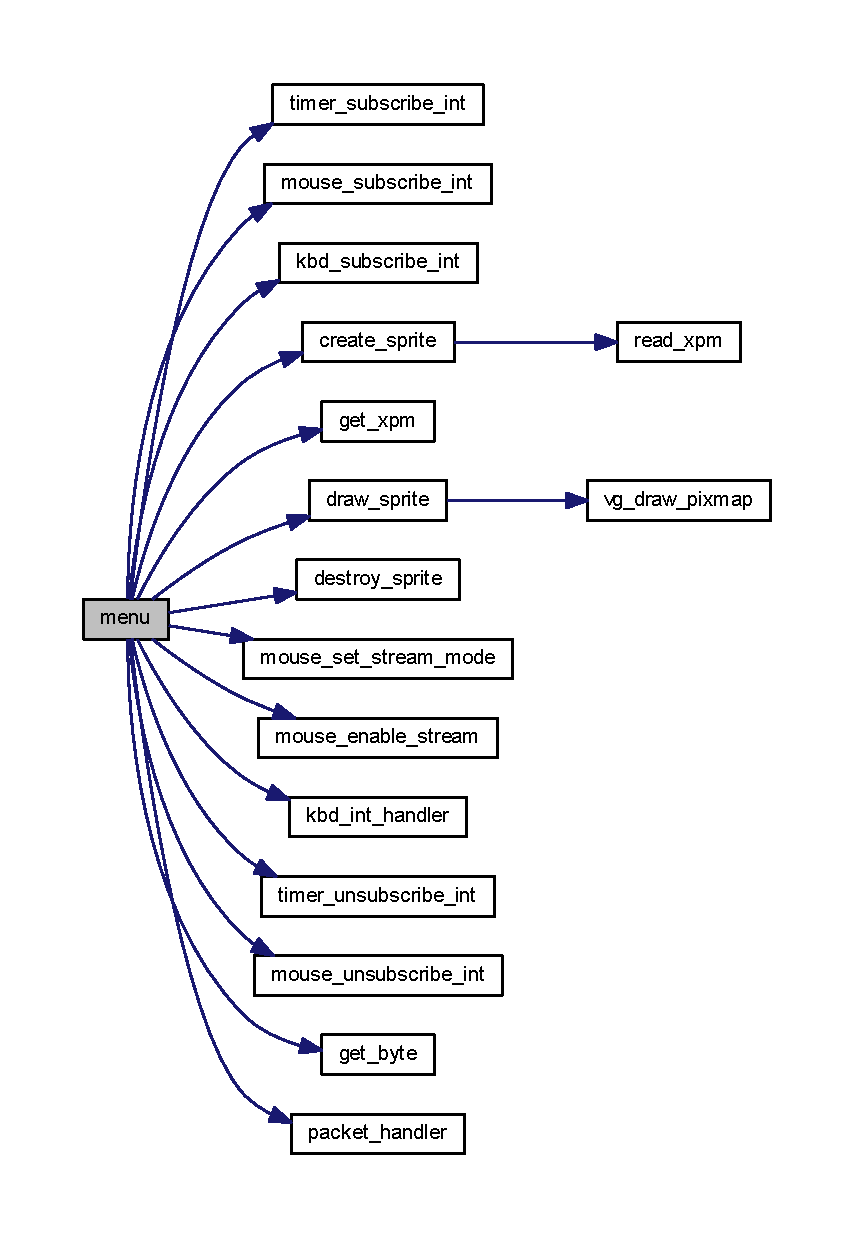
\includegraphics[width=350pt]{group__game_ga792d3a7c31488479811f72b787f85e4d_cgraph}
\end{center}
\end{figure}


\hypertarget{group__game_ga8273bb9d5ec414429bd897d7c95a1303}{}\index{game@{game}!player\+\_\+wins@{player\+\_\+wins}}
\index{player\+\_\+wins@{player\+\_\+wins}!game@{game}}
\subsubsection[{player\+\_\+wins(char $\ast$video\+\_\+mem, int player)}]{\setlength{\rightskip}{0pt plus 5cm}void player\+\_\+wins (
\begin{DoxyParamCaption}
\item[{char $\ast$}]{video\+\_\+mem, }
\item[{int}]{player}
\end{DoxyParamCaption}
)}\label{group__game_ga8273bb9d5ec414429bd897d7c95a1303}


Function for displaying the winner of the game. 

Responsible for displaying the player that took the less amount of time to complete its turn.


\begin{DoxyParams}{Parameters}
{\em video\+\_\+mem} & virtual address V\+R\+A\+M was mapped to. \\
\hline
{\em player} & number of the player that won the game. \\
\hline
\end{DoxyParams}


Here is the call graph for this function\+:\nopagebreak
\begin{figure}[H]
\begin{center}
\leavevmode
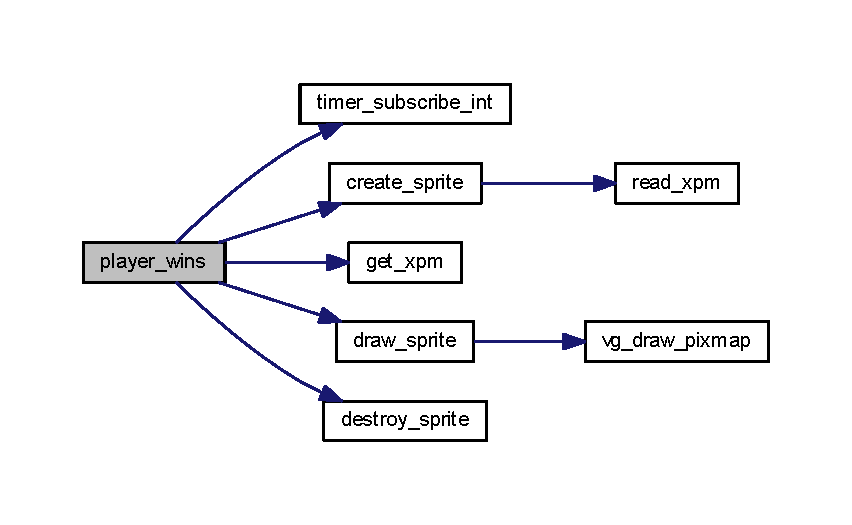
\includegraphics[width=350pt]{group__game_ga8273bb9d5ec414429bd897d7c95a1303_cgraph}
\end{center}
\end{figure}



\hypertarget{group__kbd}{}\section{kbd}
\label{group__kbd}\index{kbd@{kbd}}
\subsection*{Functions}
\begin{DoxyCompactItemize}
\item 
int \hyperlink{group__kbd_ga77e2ed8f53e0fae3f4005fa26c6d2692}{kbd\+\_\+subscribe\+\_\+int} ()
\begin{DoxyCompactList}\small\item\em Subscribes to the keyboard\textquotesingle{}s interrupts. \end{DoxyCompactList}\item 
int \hyperlink{group__kbd_gab9eea51549744bca5c5c923b388bb4ee}{timer\+\_\+unsubscribe\+\_\+int} ()
\begin{DoxyCompactList}\small\item\em Unsubscribes from the keyboard\textquotesingle{}s interrupts. \end{DoxyCompactList}\item 
int \hyperlink{group__kbd_ga76c3491bce9f85cce38e6af329b94d15}{kbd\+\_\+int\+\_\+handler} ()
\begin{DoxyCompactList}\small\item\em Unsubscribes from the keyboard\textquotesingle{}s interrupts. \end{DoxyCompactList}\end{DoxyCompactItemize}


\subsection{Detailed Description}
Functions related to the keyboard. 

\subsection{Function Documentation}
\hypertarget{group__kbd_ga76c3491bce9f85cce38e6af329b94d15}{}\index{kbd@{kbd}!kbd\+\_\+int\+\_\+handler@{kbd\+\_\+int\+\_\+handler}}
\index{kbd\+\_\+int\+\_\+handler@{kbd\+\_\+int\+\_\+handler}!kbd@{kbd}}
\subsubsection[{kbd\+\_\+int\+\_\+handler()}]{\setlength{\rightskip}{0pt plus 5cm}int kbd\+\_\+int\+\_\+handler (
\begin{DoxyParamCaption}
{}
\end{DoxyParamCaption}
)}\label{group__kbd_ga76c3491bce9f85cce38e6af329b94d15}


Unsubscribes from the keyboard\textquotesingle{}s interrupts. 

\begin{DoxyReturn}{Returns}
0 if successful. -\/1 if not. 
\end{DoxyReturn}


Here is the caller graph for this function\+:
% FIG 0


\hypertarget{group__kbd_ga77e2ed8f53e0fae3f4005fa26c6d2692}{}\index{kbd@{kbd}!kbd\+\_\+subscribe\+\_\+int@{kbd\+\_\+subscribe\+\_\+int}}
\index{kbd\+\_\+subscribe\+\_\+int@{kbd\+\_\+subscribe\+\_\+int}!kbd@{kbd}}
\subsubsection[{kbd\+\_\+subscribe\+\_\+int()}]{\setlength{\rightskip}{0pt plus 5cm}int kbd\+\_\+subscribe\+\_\+int (
\begin{DoxyParamCaption}
{}
\end{DoxyParamCaption}
)}\label{group__kbd_ga77e2ed8f53e0fae3f4005fa26c6d2692}


Subscribes to the keyboard\textquotesingle{}s interrupts. 

\begin{DoxyReturn}{Returns}
the keyboard\textquotesingle{}s hook bit if successful. -\/1 if not. 
\end{DoxyReturn}


Here is the caller graph for this function\+:
% FIG 1


\hypertarget{group__kbd_gab9eea51549744bca5c5c923b388bb4ee}{}\index{kbd@{kbd}!timer\+\_\+unsubscribe\+\_\+int@{timer\+\_\+unsubscribe\+\_\+int}}
\index{timer\+\_\+unsubscribe\+\_\+int@{timer\+\_\+unsubscribe\+\_\+int}!kbd@{kbd}}
\subsubsection[{timer\+\_\+unsubscribe\+\_\+int()}]{\setlength{\rightskip}{0pt plus 5cm}int timer\+\_\+unsubscribe\+\_\+int (
\begin{DoxyParamCaption}
{}
\end{DoxyParamCaption}
)}\label{group__kbd_gab9eea51549744bca5c5c923b388bb4ee}


Unsubscribes from the keyboard\textquotesingle{}s interrupts. 

\begin{DoxyReturn}{Returns}
0 if successful. -\/1 if not. 
\end{DoxyReturn}


Here is the caller graph for this function\+:
% FIG 2



\hypertarget{group__lmlib}{}\section{lmlib}
\label{group__lmlib}\index{lmlib@{lmlib}}
\subsection*{Data Structures}
\begin{DoxyCompactItemize}
\item 
struct \hyperlink{structmmap__t}{mmap\+\_\+t}
\end{DoxyCompactItemize}
\subsection*{Functions}
\begin{DoxyCompactItemize}
\item 
void $\ast$ \hyperlink{group__lmlib_ga00a9c17c01e794a6bfc80fc5c6ab1ed1}{lm\+\_\+init} (void)
\begin{DoxyCompactList}\small\item\em Initializes the low memory area, the region up to the 1 M\+Byte physical address, by mapping it on the process\textquotesingle{} physical memory address. \end{DoxyCompactList}\item 
void $\ast$ \hyperlink{group__lmlib_gae45d971ce2ffcf4dc2677eba033a92cd}{lm\+\_\+alloc} (unsigned long size, \hyperlink{structmmap__t}{mmap\+\_\+t} $\ast$map)
\begin{DoxyCompactList}\small\item\em Allocates a memory block in low memory area with the specified size. \end{DoxyCompactList}\item 
void \hyperlink{group__lmlib_ga73e89d9c297b7390021fb545513579c6}{lm\+\_\+free} (\hyperlink{structmmap__t}{mmap\+\_\+t} $\ast$map)
\begin{DoxyCompactList}\small\item\em Frees a memory block in the low memory area, previously allocated using \hyperlink{group__lmlib_gae45d971ce2ffcf4dc2677eba033a92cd}{lm\+\_\+alloc()} \end{DoxyCompactList}\end{DoxyCompactItemize}
\subsection*{Variables}
\begin{DoxyCompactItemize}
\item 
\hypertarget{group__lmlib_gab7a85fe0db943529016cf606e3a7167f}{}phys\+\_\+bytes \hyperlink{group__lmlib_gab7a85fe0db943529016cf606e3a7167f}{phys}\label{group__lmlib_gab7a85fe0db943529016cf606e3a7167f}

\begin{DoxyCompactList}\small\item\em physical address \end{DoxyCompactList}\item 
\hypertarget{group__lmlib_ga6a0ea2231d30f2b025e0c4b9f12dd6db}{}void $\ast$ \hyperlink{group__lmlib_ga6a0ea2231d30f2b025e0c4b9f12dd6db}{virtual}\label{group__lmlib_ga6a0ea2231d30f2b025e0c4b9f12dd6db}

\begin{DoxyCompactList}\small\item\em virtual address \end{DoxyCompactList}\item 
\hypertarget{group__lmlib_ga1e1268d164c38e4f8a4f4eb9058b0601}{}unsigned long \hyperlink{group__lmlib_ga1e1268d164c38e4f8a4f4eb9058b0601}{size}\label{group__lmlib_ga1e1268d164c38e4f8a4f4eb9058b0601}

\begin{DoxyCompactList}\small\item\em size of memory region \end{DoxyCompactList}\end{DoxyCompactItemize}


\subsection{Detailed Description}
Functions related to low memory (first 1 M\+B of physical memory), required for B\+I\+O\+S 

\subsection{Function Documentation}
\hypertarget{group__lmlib_gae45d971ce2ffcf4dc2677eba033a92cd}{}\index{lmlib@{lmlib}!lm\+\_\+alloc@{lm\+\_\+alloc}}
\index{lm\+\_\+alloc@{lm\+\_\+alloc}!lmlib@{lmlib}}
\subsubsection[{lm\+\_\+alloc(unsigned long size, mmap\+\_\+t $\ast$map)}]{\setlength{\rightskip}{0pt plus 5cm}void$\ast$ lm\+\_\+alloc (
\begin{DoxyParamCaption}
\item[{unsigned long}]{size, }
\item[{{\bf mmap\+\_\+t} $\ast$}]{map}
\end{DoxyParamCaption}
)}\label{group__lmlib_gae45d971ce2ffcf4dc2677eba033a92cd}


Allocates a memory block in low memory area with the specified size. 

Allocates a memory block in the region up to the 1 M\+Byte physical address with the input size. Initializes the input \hyperlink{structmmap__t}{mmap\+\_\+t} struct with the maping information, which can be read but must not be modified.


\begin{DoxyParams}{Parameters}
{\em size} & size of the memory block to allocate \\
\hline
{\em map} & pointer to \hyperlink{structmmap__t}{mmap\+\_\+t} data structure, which represents the memory map \\
\hline
\end{DoxyParams}
\begin{DoxyReturn}{Returns}
the virtual address of the memory block on success, N\+U\+L\+L otherwise 
\end{DoxyReturn}


Here is the caller graph for this function\+:
% FIG 0


\hypertarget{group__lmlib_ga73e89d9c297b7390021fb545513579c6}{}\index{lmlib@{lmlib}!lm\+\_\+free@{lm\+\_\+free}}
\index{lm\+\_\+free@{lm\+\_\+free}!lmlib@{lmlib}}
\subsubsection[{lm\+\_\+free(mmap\+\_\+t $\ast$map)}]{\setlength{\rightskip}{0pt plus 5cm}void lm\+\_\+free (
\begin{DoxyParamCaption}
\item[{{\bf mmap\+\_\+t} $\ast$}]{map}
\end{DoxyParamCaption}
)}\label{group__lmlib_ga73e89d9c297b7390021fb545513579c6}


Frees a memory block in the low memory area, previously allocated using \hyperlink{group__lmlib_gae45d971ce2ffcf4dc2677eba033a92cd}{lm\+\_\+alloc()} 

Frees a memory block in the region up to the 1 M\+Byte physical addess, previously allocated using \hyperlink{group__lmlib_gae45d971ce2ffcf4dc2677eba033a92cd}{lm\+\_\+alloc()}. Takes as input the address of the \hyperlink{structmmap__t}{mmap\+\_\+t} structure that was passed to \hyperlink{group__lmlib_gae45d971ce2ffcf4dc2677eba033a92cd}{lm\+\_\+alloc()}, and that must have not been modified since.


\begin{DoxyParams}{Parameters}
{\em map} & pointer to \hyperlink{structmmap__t}{mmap\+\_\+t} data structure of the block being freed \\
\hline
\end{DoxyParams}


Here is the caller graph for this function\+:
% FIG 1


\hypertarget{group__lmlib_ga00a9c17c01e794a6bfc80fc5c6ab1ed1}{}\index{lmlib@{lmlib}!lm\+\_\+init@{lm\+\_\+init}}
\index{lm\+\_\+init@{lm\+\_\+init}!lmlib@{lmlib}}
\subsubsection[{lm\+\_\+init(void)}]{\setlength{\rightskip}{0pt plus 5cm}void$\ast$ lm\+\_\+init (
\begin{DoxyParamCaption}
\item[{void}]{}
\end{DoxyParamCaption}
)}\label{group__lmlib_ga00a9c17c01e794a6bfc80fc5c6ab1ed1}


Initializes the low memory area, the region up to the 1 M\+Byte physical address, by mapping it on the process\textquotesingle{} physical memory address. 

\begin{DoxyReturn}{Returns}
virtual address on which the first 1 Mi\+B was mapped, N\+U\+L\+L upon failure 
\end{DoxyReturn}


Here is the caller graph for this function\+:
% FIG 2



\hypertarget{group__mouse}{}\section{mouse}
\label{group__mouse}\index{mouse@{mouse}}
\subsection*{Functions}
\begin{DoxyCompactItemize}
\item 
int \hyperlink{group__mouse_ga99506573209b197b84ee22a228b89fbd}{mouse\+\_\+subscribe\+\_\+int} ()
\begin{DoxyCompactList}\small\item\em Subscribes to the mouse\textquotesingle{}s interrupts. \end{DoxyCompactList}\item 
int \hyperlink{group__mouse_ga685ad2706aca36d9869a30a19b9f446a}{mouse\+\_\+unsubscribe\+\_\+int} ()
\begin{DoxyCompactList}\small\item\em Unsubscribes from the mouse\textquotesingle{}s interrupts. \end{DoxyCompactList}\item 
int \hyperlink{group__mouse_ga16a521d1919cbd8f434d8b5d535a639b}{mouse\+\_\+set\+\_\+stream\+\_\+mode} ()
\begin{DoxyCompactList}\small\item\em Sends the Set Stream Mode command to port 0x64. \end{DoxyCompactList}\item 
int \hyperlink{group__mouse_ga6d00dfd9c62a4446f67caea39b64d463}{mouse\+\_\+enable\+\_\+stream} ()
\begin{DoxyCompactList}\small\item\em Sends the Enable Sending Data Packets command to port 0x64. \end{DoxyCompactList}\item 
int \hyperlink{group__mouse_gaff2fd99bd9285fa0fc166788f9cc7569}{mouse\+\_\+status\+\_\+request} ()
\begin{DoxyCompactList}\small\item\em Sends the Status Request command to port 0x64. \end{DoxyCompactList}\item 
long \hyperlink{group__mouse_ga59b282691a2a3edde462f7b36351a74a}{get\+\_\+byte} ()
\begin{DoxyCompactList}\small\item\em Receives the data in port 0x60. \end{DoxyCompactList}\item 
int \hyperlink{group__mouse_ga04bd9f2c1818e56a4604e290a068842b}{packet\+\_\+handler} (char data\+\_\+packet\mbox{[}$\,$\mbox{]}, \hyperlink{struct_sprite}{Sprite} $\ast$sprite, char $\ast$video\+\_\+mem)
\begin{DoxyCompactList}\small\item\em Receives a mouse data packet and updates the sprite\textquotesingle{}s coordinates accordingly. \end{DoxyCompactList}\end{DoxyCompactItemize}


\subsection{Detailed Description}
Functions related to the mouse. 

\subsection{Function Documentation}
\hypertarget{group__mouse_ga59b282691a2a3edde462f7b36351a74a}{}\index{mouse@{mouse}!get\+\_\+byte@{get\+\_\+byte}}
\index{get\+\_\+byte@{get\+\_\+byte}!mouse@{mouse}}
\subsubsection[{get\+\_\+byte()}]{\setlength{\rightskip}{0pt plus 5cm}long get\+\_\+byte (
\begin{DoxyParamCaption}
{}
\end{DoxyParamCaption}
)}\label{group__mouse_ga59b282691a2a3edde462f7b36351a74a}


Receives the data in port 0x60. 

\begin{DoxyReturn}{Returns}
the date when successful. 
\end{DoxyReturn}


Here is the caller graph for this function\+:
% FIG 0


\hypertarget{group__mouse_ga6d00dfd9c62a4446f67caea39b64d463}{}\index{mouse@{mouse}!mouse\+\_\+enable\+\_\+stream@{mouse\+\_\+enable\+\_\+stream}}
\index{mouse\+\_\+enable\+\_\+stream@{mouse\+\_\+enable\+\_\+stream}!mouse@{mouse}}
\subsubsection[{mouse\+\_\+enable\+\_\+stream()}]{\setlength{\rightskip}{0pt plus 5cm}int mouse\+\_\+enable\+\_\+stream (
\begin{DoxyParamCaption}
{}
\end{DoxyParamCaption}
)}\label{group__mouse_ga6d00dfd9c62a4446f67caea39b64d463}


Sends the Enable Sending Data Packets command to port 0x64. 

\begin{DoxyReturn}{Returns}
0 if successful. 1 if not. 
\end{DoxyReturn}


Here is the caller graph for this function\+:
% FIG 1


\hypertarget{group__mouse_ga16a521d1919cbd8f434d8b5d535a639b}{}\index{mouse@{mouse}!mouse\+\_\+set\+\_\+stream\+\_\+mode@{mouse\+\_\+set\+\_\+stream\+\_\+mode}}
\index{mouse\+\_\+set\+\_\+stream\+\_\+mode@{mouse\+\_\+set\+\_\+stream\+\_\+mode}!mouse@{mouse}}
\subsubsection[{mouse\+\_\+set\+\_\+stream\+\_\+mode()}]{\setlength{\rightskip}{0pt plus 5cm}int mouse\+\_\+set\+\_\+stream\+\_\+mode (
\begin{DoxyParamCaption}
{}
\end{DoxyParamCaption}
)}\label{group__mouse_ga16a521d1919cbd8f434d8b5d535a639b}


Sends the Set Stream Mode command to port 0x64. 

\begin{DoxyReturn}{Returns}
0 if successful. 1 if not. 
\end{DoxyReturn}


Here is the caller graph for this function\+:
% FIG 2


\hypertarget{group__mouse_gaff2fd99bd9285fa0fc166788f9cc7569}{}\index{mouse@{mouse}!mouse\+\_\+status\+\_\+request@{mouse\+\_\+status\+\_\+request}}
\index{mouse\+\_\+status\+\_\+request@{mouse\+\_\+status\+\_\+request}!mouse@{mouse}}
\subsubsection[{mouse\+\_\+status\+\_\+request()}]{\setlength{\rightskip}{0pt plus 5cm}int mouse\+\_\+status\+\_\+request (
\begin{DoxyParamCaption}
{}
\end{DoxyParamCaption}
)}\label{group__mouse_gaff2fd99bd9285fa0fc166788f9cc7569}


Sends the Status Request command to port 0x64. 

\begin{DoxyReturn}{Returns}
0 if successful. 1 if not. 
\end{DoxyReturn}
\hypertarget{group__mouse_ga99506573209b197b84ee22a228b89fbd}{}\index{mouse@{mouse}!mouse\+\_\+subscribe\+\_\+int@{mouse\+\_\+subscribe\+\_\+int}}
\index{mouse\+\_\+subscribe\+\_\+int@{mouse\+\_\+subscribe\+\_\+int}!mouse@{mouse}}
\subsubsection[{mouse\+\_\+subscribe\+\_\+int()}]{\setlength{\rightskip}{0pt plus 5cm}int mouse\+\_\+subscribe\+\_\+int (
\begin{DoxyParamCaption}
{}
\end{DoxyParamCaption}
)}\label{group__mouse_ga99506573209b197b84ee22a228b89fbd}


Subscribes to the mouse\textquotesingle{}s interrupts. 

\begin{DoxyReturn}{Returns}
the mouse\textquotesingle{}s hook bit if successful. -\/1 if not. 
\end{DoxyReturn}


Here is the caller graph for this function\+:
% FIG 3


\hypertarget{group__mouse_ga685ad2706aca36d9869a30a19b9f446a}{}\index{mouse@{mouse}!mouse\+\_\+unsubscribe\+\_\+int@{mouse\+\_\+unsubscribe\+\_\+int}}
\index{mouse\+\_\+unsubscribe\+\_\+int@{mouse\+\_\+unsubscribe\+\_\+int}!mouse@{mouse}}
\subsubsection[{mouse\+\_\+unsubscribe\+\_\+int()}]{\setlength{\rightskip}{0pt plus 5cm}int mouse\+\_\+unsubscribe\+\_\+int (
\begin{DoxyParamCaption}
{}
\end{DoxyParamCaption}
)}\label{group__mouse_ga685ad2706aca36d9869a30a19b9f446a}


Unsubscribes from the mouse\textquotesingle{}s interrupts. 

\begin{DoxyReturn}{Returns}
0 if successful. -\/1 if not. 
\end{DoxyReturn}


Here is the caller graph for this function\+:
% FIG 4


\hypertarget{group__mouse_ga04bd9f2c1818e56a4604e290a068842b}{}\index{mouse@{mouse}!packet\+\_\+handler@{packet\+\_\+handler}}
\index{packet\+\_\+handler@{packet\+\_\+handler}!mouse@{mouse}}
\subsubsection[{packet\+\_\+handler(char data\+\_\+packet[], Sprite $\ast$sprite, char $\ast$video\+\_\+mem)}]{\setlength{\rightskip}{0pt plus 5cm}int packet\+\_\+handler (
\begin{DoxyParamCaption}
\item[{char}]{data\+\_\+packet\mbox{[}$\,$\mbox{]}, }
\item[{{\bf Sprite} $\ast$}]{sprite, }
\item[{char $\ast$}]{video\+\_\+mem}
\end{DoxyParamCaption}
)}\label{group__mouse_ga04bd9f2c1818e56a4604e290a068842b}


Receives a mouse data packet and updates the sprite\textquotesingle{}s coordinates accordingly. 


\begin{DoxyParams}{Parameters}
{\em data\+\_\+packet} & array containing the data from the mouse. \\
\hline
{\em sprite} & pointer to a sprite. \\
\hline
{\em video\+\_\+mem} & virtual address V\+R\+A\+M was mapped to.\\
\hline
\end{DoxyParams}
\begin{DoxyReturn}{Returns}
1 if the left button is pressed. 0 if not. 
\end{DoxyReturn}


Here is the caller graph for this function\+:
% FIG 5



\hypertarget{group__sprite}{}\section{sprite}
\label{group__sprite}\index{sprite@{sprite}}
\subsection*{Data Structures}
\begin{DoxyCompactItemize}
\item 
struct \hyperlink{struct_sprite}{Sprite}
\end{DoxyCompactItemize}
\subsection*{Variables}
\begin{DoxyCompactItemize}
\item 
\hypertarget{group__sprite_ga6150e0515f7202e2fb518f7206ed97dc}{}int {\bfseries x}\label{group__sprite_ga6150e0515f7202e2fb518f7206ed97dc}

\item 
int \hyperlink{group__sprite_ga0a2f84ed7838f07779ae24c5a9086d33}{y}
\item 
int \hyperlink{group__sprite_ga2474a5474cbff19523a51eb1de01cda4}{width}
\item 
int \hyperlink{group__sprite_gad12fc34ce789bce6c8a05d8a17138534}{height}
\item 
int \hyperlink{group__sprite_ga56d83ad8a1afb318706057c1ec72f797}{x\+\_\+speed}
\item 
int \hyperlink{group__sprite_ga081c2d7f9619a32bd806baa1831ce1c1}{y\+\_\+speed}
\item 
int \hyperlink{group__sprite_gad427edc16087f64ef18fb771dd34cc0b}{jumping}
\item 
int \hyperlink{group__sprite_ga44675e845628c15d8a696990a9494d04}{inplatform}
\item 
char $\ast$ \hyperlink{group__sprite_ga7b00b1bfd666e26484471bd17a74eaa9}{map}
\end{DoxyCompactItemize}
\subsection*{Sprite}
\begin{DoxyCompactItemize}
\item 
\hyperlink{struct_sprite}{Sprite} $\ast$ \hyperlink{group__sprite_ga585fbaeb1d5f34bb4e1393e7e99697dd}{create\+\_\+sprite} (char $\ast$pic\mbox{[}$\,$\mbox{]}, unsigned short x, unsigned short y)
\begin{DoxyCompactList}\small\item\em Creates a sprite. \end{DoxyCompactList}\item 
int \hyperlink{group__sprite_ga65b342bdee0447b4d253a3fcfc95d78b}{draw\+\_\+sprite} (\hyperlink{struct_sprite}{Sprite} $\ast$sp, char $\ast$video\+\_\+mem)
\begin{DoxyCompactList}\small\item\em Draws a sprite. \end{DoxyCompactList}\item 
int \hyperlink{group__sprite_ga8446db36e642f6bb7e0e566f0fac9637}{move\+\_\+sprite} (\hyperlink{struct_sprite}{Sprite} $\ast$sp, unsigned short h\+\_\+res, unsigned short v\+\_\+res, char $\ast$video\+\_\+mem)
\begin{DoxyCompactList}\small\item\em Moves a sprite. \end{DoxyCompactList}\item 
int \hyperlink{group__sprite_gab9af15d14a3cb2f3f290be7355fbdb77}{move\+\_\+shot} (\hyperlink{struct_sprite}{Sprite} $\ast$sp, \hyperlink{struct_sprite}{Sprite} $\ast$p, unsigned short h\+\_\+res, unsigned short v\+\_\+res, char $\ast$video\+\_\+mem)
\begin{DoxyCompactList}\small\item\em Moves a shot sprite. \end{DoxyCompactList}\item 
void \hyperlink{group__sprite_ga4dd652976ab61cba06875d87e52df12f}{set\+\_\+x\+\_\+speed\+\_\+sprite} (\hyperlink{struct_sprite}{Sprite} $\ast$sp, int x\+\_\+speed)
\begin{DoxyCompactList}\small\item\em Sets a sprite\textquotesingle{}s horizontal speed to the specified. \end{DoxyCompactList}\item 
void \hyperlink{group__sprite_ga4ca599f2889585f0c7a78ec6622d6928}{set\+\_\+y\+\_\+speed\+\_\+sprite} (\hyperlink{struct_sprite}{Sprite} $\ast$sp, int y\+\_\+speed)
\begin{DoxyCompactList}\small\item\em Sets a sprite\textquotesingle{}s vertical speed to the specified. \end{DoxyCompactList}\item 
void \hyperlink{group__sprite_gaf16c6befaac9ffb673b9e3c798d542ed}{destroy\+\_\+sprite} (\hyperlink{struct_sprite}{Sprite} $\ast$sp)
\begin{DoxyCompactList}\small\item\em Frees the memory occupied by the sprite. \end{DoxyCompactList}\end{DoxyCompactItemize}


\subsection{Detailed Description}
Functions related to the objects to be displayed on screen. 

\subsection{Function Documentation}
\hypertarget{group__sprite_ga585fbaeb1d5f34bb4e1393e7e99697dd}{}\index{sprite@{sprite}!create\+\_\+sprite@{create\+\_\+sprite}}
\index{create\+\_\+sprite@{create\+\_\+sprite}!sprite@{sprite}}
\subsubsection[{create\+\_\+sprite(char $\ast$pic[], unsigned short x, unsigned short y)}]{\setlength{\rightskip}{0pt plus 5cm}{\bf Sprite}$\ast$ create\+\_\+sprite (
\begin{DoxyParamCaption}
\item[{char $\ast$}]{pic\mbox{[}$\,$\mbox{]}, }
\item[{unsigned short}]{x, }
\item[{unsigned short}]{y}
\end{DoxyParamCaption}
)}\label{group__sprite_ga585fbaeb1d5f34bb4e1393e7e99697dd}


Creates a sprite. 

Creates a sprite using the pixmap and coordinates given. The rest of the parameters are initialized to 0.


\begin{DoxyParams}{Parameters}
{\em pic} & pointer to pixmap. \\
\hline
{\em x} & coordinate for the sprite. \\
\hline
{\em y} & coordinate for the sprite \\
\hline
\end{DoxyParams}
\begin{DoxyReturn}{Returns}
pointer to the created sprite. 
\end{DoxyReturn}


Here is the call graph for this function\+:\nopagebreak
\begin{figure}[H]
\begin{center}
\leavevmode
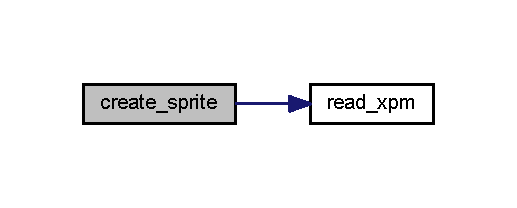
\includegraphics[width=248pt]{group__sprite_ga585fbaeb1d5f34bb4e1393e7e99697dd_cgraph}
\end{center}
\end{figure}




Here is the caller graph for this function\+:\nopagebreak
\begin{figure}[H]
\begin{center}
\leavevmode
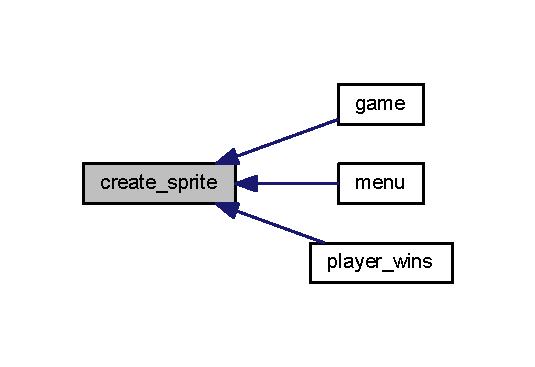
\includegraphics[width=257pt]{group__sprite_ga585fbaeb1d5f34bb4e1393e7e99697dd_icgraph}
\end{center}
\end{figure}


\hypertarget{group__sprite_gaf16c6befaac9ffb673b9e3c798d542ed}{}\index{sprite@{sprite}!destroy\+\_\+sprite@{destroy\+\_\+sprite}}
\index{destroy\+\_\+sprite@{destroy\+\_\+sprite}!sprite@{sprite}}
\subsubsection[{destroy\+\_\+sprite(\+Sprite $\ast$sp)}]{\setlength{\rightskip}{0pt plus 5cm}void destroy\+\_\+sprite (
\begin{DoxyParamCaption}
\item[{{\bf Sprite} $\ast$}]{sp}
\end{DoxyParamCaption}
)}\label{group__sprite_gaf16c6befaac9ffb673b9e3c798d542ed}


Frees the memory occupied by the sprite. 


\begin{DoxyParams}{Parameters}
{\em sp} & pointer to a sprite. \\
\hline
\end{DoxyParams}


Here is the caller graph for this function\+:\nopagebreak
\begin{figure}[H]
\begin{center}
\leavevmode
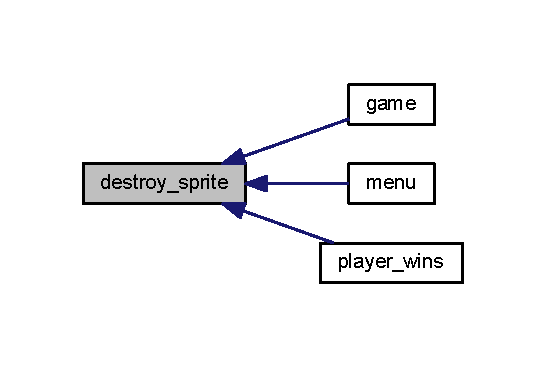
\includegraphics[width=262pt]{group__sprite_gaf16c6befaac9ffb673b9e3c798d542ed_icgraph}
\end{center}
\end{figure}


\hypertarget{group__sprite_ga65b342bdee0447b4d253a3fcfc95d78b}{}\index{sprite@{sprite}!draw\+\_\+sprite@{draw\+\_\+sprite}}
\index{draw\+\_\+sprite@{draw\+\_\+sprite}!sprite@{sprite}}
\subsubsection[{draw\+\_\+sprite(\+Sprite $\ast$sp, char $\ast$video\+\_\+mem)}]{\setlength{\rightskip}{0pt plus 5cm}int draw\+\_\+sprite (
\begin{DoxyParamCaption}
\item[{{\bf Sprite} $\ast$}]{sp, }
\item[{char $\ast$}]{video\+\_\+mem}
\end{DoxyParamCaption}
)}\label{group__sprite_ga65b342bdee0447b4d253a3fcfc95d78b}


Draws a sprite. 

Draws a sprite in the buffer given.


\begin{DoxyParams}{Parameters}
{\em sp} & pointer to a sprite. \\
\hline
{\em video\+\_\+mem} & pointer to a buffer. \\
\hline
\end{DoxyParams}
\begin{DoxyReturn}{Returns}
0 if the sprites fits in the buffer. 1 if not. 
\end{DoxyReturn}


Here is the call graph for this function\+:\nopagebreak
\begin{figure}[H]
\begin{center}
\leavevmode
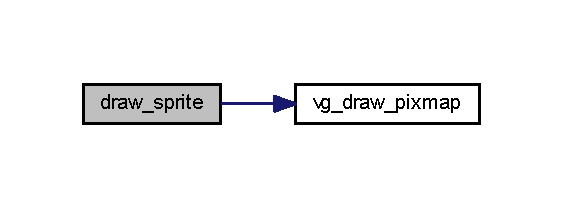
\includegraphics[width=270pt]{group__sprite_ga65b342bdee0447b4d253a3fcfc95d78b_cgraph}
\end{center}
\end{figure}




Here is the caller graph for this function\+:\nopagebreak
\begin{figure}[H]
\begin{center}
\leavevmode
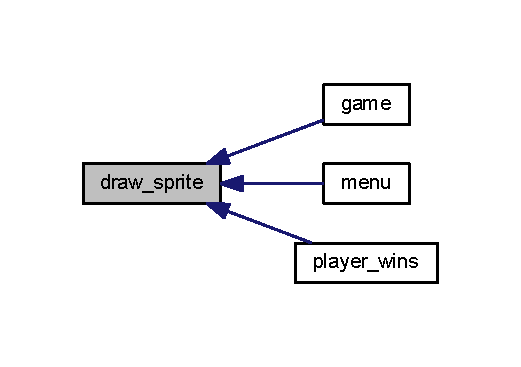
\includegraphics[width=250pt]{group__sprite_ga65b342bdee0447b4d253a3fcfc95d78b_icgraph}
\end{center}
\end{figure}


\hypertarget{group__sprite_gab9af15d14a3cb2f3f290be7355fbdb77}{}\index{sprite@{sprite}!move\+\_\+shot@{move\+\_\+shot}}
\index{move\+\_\+shot@{move\+\_\+shot}!sprite@{sprite}}
\subsubsection[{move\+\_\+shot(\+Sprite $\ast$sp, Sprite $\ast$p, unsigned short h\+\_\+res, unsigned short v\+\_\+res, char $\ast$video\+\_\+mem)}]{\setlength{\rightskip}{0pt plus 5cm}int move\+\_\+shot (
\begin{DoxyParamCaption}
\item[{{\bf Sprite} $\ast$}]{sp, }
\item[{{\bf Sprite} $\ast$}]{p, }
\item[{unsigned short}]{h\+\_\+res, }
\item[{unsigned short}]{v\+\_\+res, }
\item[{char $\ast$}]{video\+\_\+mem}
\end{DoxyParamCaption}
)}\label{group__sprite_gab9af15d14a3cb2f3f290be7355fbdb77}


Moves a shot sprite. 

Moves a shot sprite, checking the collisions with the borders and other sprites. Updates its position. Also checks if it hits the other player.


\begin{DoxyParams}{Parameters}
{\em sp} & pointer to the shot sprite. \\
\hline
{\em p} & pointer to the player to hit sprite. \\
\hline
{\em h\+\_\+res} & width of the buffer. \\
\hline
{\em v\+\_\+res} & height of the buffer. \\
\hline
{\em video\+\_\+mem} & pointer to a buffer. \\
\hline
\end{DoxyParams}
\begin{DoxyReturn}{Returns}
1-\/4 if the sprite collides with a border. 5 if it collides with a sprite other that the player\textquotesingle{}s. 6 if it collides with the player. 0 if there are no collisions. 
\end{DoxyReturn}


Here is the caller graph for this function\+:\nopagebreak
\begin{figure}[H]
\begin{center}
\leavevmode
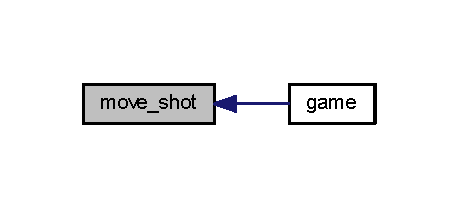
\includegraphics[width=220pt]{group__sprite_gab9af15d14a3cb2f3f290be7355fbdb77_icgraph}
\end{center}
\end{figure}


\hypertarget{group__sprite_ga8446db36e642f6bb7e0e566f0fac9637}{}\index{sprite@{sprite}!move\+\_\+sprite@{move\+\_\+sprite}}
\index{move\+\_\+sprite@{move\+\_\+sprite}!sprite@{sprite}}
\subsubsection[{move\+\_\+sprite(\+Sprite $\ast$sp, unsigned short h\+\_\+res, unsigned short v\+\_\+res, char $\ast$video\+\_\+mem)}]{\setlength{\rightskip}{0pt plus 5cm}int move\+\_\+sprite (
\begin{DoxyParamCaption}
\item[{{\bf Sprite} $\ast$}]{sp, }
\item[{unsigned short}]{h\+\_\+res, }
\item[{unsigned short}]{v\+\_\+res, }
\item[{char $\ast$}]{video\+\_\+mem}
\end{DoxyParamCaption}
)}\label{group__sprite_ga8446db36e642f6bb7e0e566f0fac9637}


Moves a sprite. 

Moves a sprite, checking the collisions with the borders and other sprites. Updates its position, jumping and inplatform.


\begin{DoxyParams}{Parameters}
{\em sp} & pointer to a sprite. \\
\hline
{\em h\+\_\+res} & width of the buffer. \\
\hline
{\em v\+\_\+res} & height of the buffer. \\
\hline
{\em video\+\_\+mem} & pointer to a buffer. \\
\hline
\end{DoxyParams}
\begin{DoxyReturn}{Returns}
1-\/4 if the sprite collides with a border. 5-\/7 if it collides with another sprite. 0 if there are no collisions. 
\end{DoxyReturn}


Here is the call graph for this function\+:\nopagebreak
\begin{figure}[H]
\begin{center}
\leavevmode
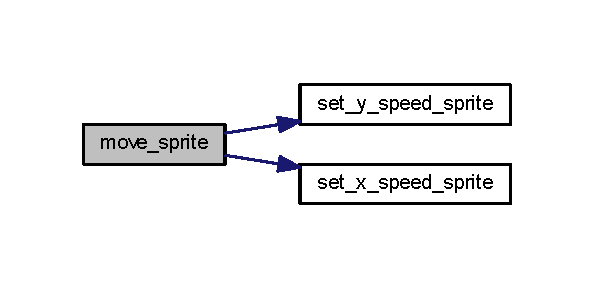
\includegraphics[width=285pt]{group__sprite_ga8446db36e642f6bb7e0e566f0fac9637_cgraph}
\end{center}
\end{figure}




Here is the caller graph for this function\+:\nopagebreak
\begin{figure}[H]
\begin{center}
\leavevmode
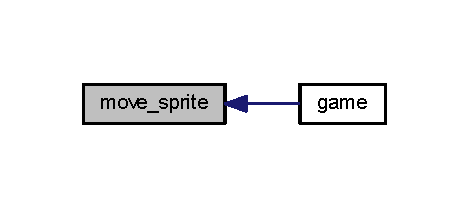
\includegraphics[width=225pt]{group__sprite_ga8446db36e642f6bb7e0e566f0fac9637_icgraph}
\end{center}
\end{figure}


\hypertarget{group__sprite_ga4dd652976ab61cba06875d87e52df12f}{}\index{sprite@{sprite}!set\+\_\+x\+\_\+speed\+\_\+sprite@{set\+\_\+x\+\_\+speed\+\_\+sprite}}
\index{set\+\_\+x\+\_\+speed\+\_\+sprite@{set\+\_\+x\+\_\+speed\+\_\+sprite}!sprite@{sprite}}
\subsubsection[{set\+\_\+x\+\_\+speed\+\_\+sprite(\+Sprite $\ast$sp, int x\+\_\+speed)}]{\setlength{\rightskip}{0pt plus 5cm}void set\+\_\+x\+\_\+speed\+\_\+sprite (
\begin{DoxyParamCaption}
\item[{{\bf Sprite} $\ast$}]{sp, }
\item[{int}]{x\+\_\+speed}
\end{DoxyParamCaption}
)}\label{group__sprite_ga4dd652976ab61cba06875d87e52df12f}


Sets a sprite\textquotesingle{}s horizontal speed to the specified. 


\begin{DoxyParams}{Parameters}
{\em sp} & pointer to a sprite. \\
\hline
{\em x\+\_\+speed} & sprite\textquotesingle{}s new x speed. \\
\hline
\end{DoxyParams}


Here is the caller graph for this function\+:\nopagebreak
\begin{figure}[H]
\begin{center}
\leavevmode
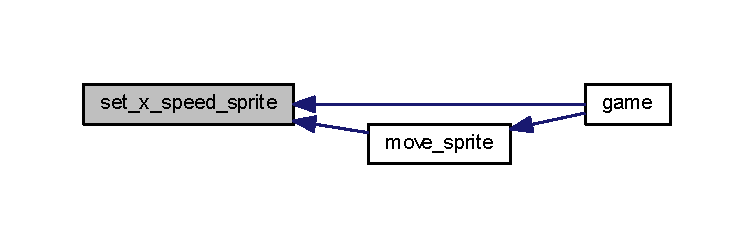
\includegraphics[width=350pt]{group__sprite_ga4dd652976ab61cba06875d87e52df12f_icgraph}
\end{center}
\end{figure}


\hypertarget{group__sprite_ga4ca599f2889585f0c7a78ec6622d6928}{}\index{sprite@{sprite}!set\+\_\+y\+\_\+speed\+\_\+sprite@{set\+\_\+y\+\_\+speed\+\_\+sprite}}
\index{set\+\_\+y\+\_\+speed\+\_\+sprite@{set\+\_\+y\+\_\+speed\+\_\+sprite}!sprite@{sprite}}
\subsubsection[{set\+\_\+y\+\_\+speed\+\_\+sprite(\+Sprite $\ast$sp, int y\+\_\+speed)}]{\setlength{\rightskip}{0pt plus 5cm}void set\+\_\+y\+\_\+speed\+\_\+sprite (
\begin{DoxyParamCaption}
\item[{{\bf Sprite} $\ast$}]{sp, }
\item[{int}]{y\+\_\+speed}
\end{DoxyParamCaption}
)}\label{group__sprite_ga4ca599f2889585f0c7a78ec6622d6928}


Sets a sprite\textquotesingle{}s vertical speed to the specified. 


\begin{DoxyParams}{Parameters}
{\em sp} & pointer to a sprite. \\
\hline
{\em y\+\_\+speed} & sprite\textquotesingle{}s new y speed. \\
\hline
\end{DoxyParams}


Here is the caller graph for this function\+:\nopagebreak
\begin{figure}[H]
\begin{center}
\leavevmode
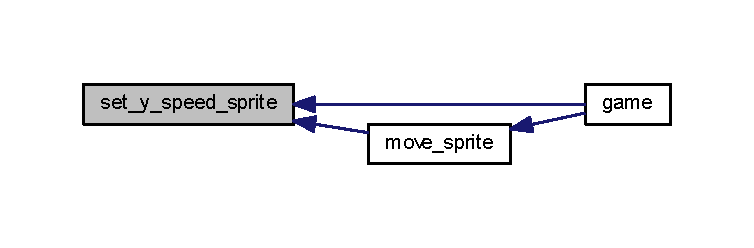
\includegraphics[width=350pt]{group__sprite_ga4ca599f2889585f0c7a78ec6622d6928_icgraph}
\end{center}
\end{figure}




\subsection{Variable Documentation}
\hypertarget{group__sprite_gad12fc34ce789bce6c8a05d8a17138534}{}\index{sprite@{sprite}!height@{height}}
\index{height@{height}!sprite@{sprite}}
\subsubsection[{height}]{\setlength{\rightskip}{0pt plus 5cm}int height}\label{group__sprite_gad12fc34ce789bce6c8a05d8a17138534}
Dimensions of the sprite. \hypertarget{group__sprite_ga44675e845628c15d8a696990a9494d04}{}\index{sprite@{sprite}!inplatform@{inplatform}}
\index{inplatform@{inplatform}!sprite@{sprite}}
\subsubsection[{inplatform}]{\setlength{\rightskip}{0pt plus 5cm}int inplatform}\label{group__sprite_ga44675e845628c15d8a696990a9494d04}
Used to track if the sprite is on a platform (1) or not (0). \hypertarget{group__sprite_gad427edc16087f64ef18fb771dd34cc0b}{}\index{sprite@{sprite}!jumping@{jumping}}
\index{jumping@{jumping}!sprite@{sprite}}
\subsubsection[{jumping}]{\setlength{\rightskip}{0pt plus 5cm}int jumping}\label{group__sprite_gad427edc16087f64ef18fb771dd34cc0b}
Used to track if the sprite is jumping (1) or not (0). \hypertarget{group__sprite_ga7b00b1bfd666e26484471bd17a74eaa9}{}\index{sprite@{sprite}!map@{map}}
\index{map@{map}!sprite@{sprite}}
\subsubsection[{map}]{\setlength{\rightskip}{0pt plus 5cm}char$\ast$ map}\label{group__sprite_ga7b00b1bfd666e26484471bd17a74eaa9}
Pointer to the pixmap of the sprite. \hypertarget{group__sprite_ga2474a5474cbff19523a51eb1de01cda4}{}\index{sprite@{sprite}!width@{width}}
\index{width@{width}!sprite@{sprite}}
\subsubsection[{width}]{\setlength{\rightskip}{0pt plus 5cm}int width}\label{group__sprite_ga2474a5474cbff19523a51eb1de01cda4}
$<$ Dimensions of the sprite. \hypertarget{group__sprite_ga56d83ad8a1afb318706057c1ec72f797}{}\index{sprite@{sprite}!x\+\_\+speed@{x\+\_\+speed}}
\index{x\+\_\+speed@{x\+\_\+speed}!sprite@{sprite}}
\subsubsection[{x\+\_\+speed}]{\setlength{\rightskip}{0pt plus 5cm}int x\+\_\+speed}\label{group__sprite_ga56d83ad8a1afb318706057c1ec72f797}
$<$ Speed of the sprite. \hypertarget{group__sprite_ga0a2f84ed7838f07779ae24c5a9086d33}{}\index{sprite@{sprite}!y@{y}}
\index{y@{y}!sprite@{sprite}}
\subsubsection[{y}]{\setlength{\rightskip}{0pt plus 5cm}int y}\label{group__sprite_ga0a2f84ed7838f07779ae24c5a9086d33}
Coordinates of the sprite. \hypertarget{group__sprite_ga081c2d7f9619a32bd806baa1831ce1c1}{}\index{sprite@{sprite}!y\+\_\+speed@{y\+\_\+speed}}
\index{y\+\_\+speed@{y\+\_\+speed}!sprite@{sprite}}
\subsubsection[{y\+\_\+speed}]{\setlength{\rightskip}{0pt plus 5cm}int y\+\_\+speed}\label{group__sprite_ga081c2d7f9619a32bd806baa1831ce1c1}
Speed of the sprite. 
\hypertarget{group__timer}{}\section{timer}
\label{group__timer}\index{timer@{timer}}
\subsection*{Functions}
\begin{DoxyCompactItemize}
\item 
int \hyperlink{group__timer_gada4efbb5c88275795526fc45f0814aa3}{timer\+\_\+set\+\_\+square} (unsigned long timer, unsigned long freq)
\begin{DoxyCompactList}\small\item\em Configures a timer to generate a square wave. \end{DoxyCompactList}\item 
int \hyperlink{group__timer_ga4c5d9f47323eda494cfd826f6d62eec9}{timer\+\_\+subscribe\+\_\+int} (void)
\begin{DoxyCompactList}\small\item\em Subscribes and enables Timer 0 interrupts. \end{DoxyCompactList}\item 
int \hyperlink{group__timer_gab9eea51549744bca5c5c923b388bb4ee}{timer\+\_\+unsubscribe\+\_\+int} ()
\begin{DoxyCompactList}\small\item\em Unsubscribes Timer 0 interrupts. \end{DoxyCompactList}\end{DoxyCompactItemize}


\subsection{Detailed Description}
Functions related to the timer. 

\subsection{Function Documentation}
\hypertarget{group__timer_gada4efbb5c88275795526fc45f0814aa3}{}\index{timer@{timer}!timer\+\_\+set\+\_\+square@{timer\+\_\+set\+\_\+square}}
\index{timer\+\_\+set\+\_\+square@{timer\+\_\+set\+\_\+square}!timer@{timer}}
\subsubsection[{timer\+\_\+set\+\_\+square(unsigned long timer, unsigned long freq)}]{\setlength{\rightskip}{0pt plus 5cm}int timer\+\_\+set\+\_\+square (
\begin{DoxyParamCaption}
\item[{unsigned long}]{timer, }
\item[{unsigned long}]{freq}
\end{DoxyParamCaption}
)}\label{group__timer_gada4efbb5c88275795526fc45f0814aa3}


Configures a timer to generate a square wave. 

Does not change the L\+S\+B (B\+C\+D/binary) of the timer\textquotesingle{}s control word.


\begin{DoxyParams}{Parameters}
{\em timer} & Timer to configure. (Ranges from 0 to 2) \\
\hline
{\em freq} & Frequency of the square wave to generate \\
\hline
\end{DoxyParams}
\begin{DoxyReturn}{Returns}
Return 0 upon success and non-\/zero otherwise 
\end{DoxyReturn}
\hypertarget{group__timer_ga4c5d9f47323eda494cfd826f6d62eec9}{}\index{timer@{timer}!timer\+\_\+subscribe\+\_\+int@{timer\+\_\+subscribe\+\_\+int}}
\index{timer\+\_\+subscribe\+\_\+int@{timer\+\_\+subscribe\+\_\+int}!timer@{timer}}
\subsubsection[{timer\+\_\+subscribe\+\_\+int(void)}]{\setlength{\rightskip}{0pt plus 5cm}int timer\+\_\+subscribe\+\_\+int (
\begin{DoxyParamCaption}
\item[{void}]{}
\end{DoxyParamCaption}
)}\label{group__timer_ga4c5d9f47323eda494cfd826f6d62eec9}


Subscribes and enables Timer 0 interrupts. 

\begin{DoxyReturn}{Returns}
Returns bit order in interrupt mask; negative value on failure 
\end{DoxyReturn}


Here is the caller graph for this function\+:
% FIG 0


\hypertarget{group__timer_gab9eea51549744bca5c5c923b388bb4ee}{}\index{timer@{timer}!timer\+\_\+unsubscribe\+\_\+int@{timer\+\_\+unsubscribe\+\_\+int}}
\index{timer\+\_\+unsubscribe\+\_\+int@{timer\+\_\+unsubscribe\+\_\+int}!timer@{timer}}
\subsubsection[{timer\+\_\+unsubscribe\+\_\+int()}]{\setlength{\rightskip}{0pt plus 5cm}int timer\+\_\+unsubscribe\+\_\+int (
\begin{DoxyParamCaption}
{}
\end{DoxyParamCaption}
)}\label{group__timer_gab9eea51549744bca5c5c923b388bb4ee}


Unsubscribes Timer 0 interrupts. 

\begin{DoxyReturn}{Returns}
Return 0 upon success and non-\/zero otherwise
\end{DoxyReturn}
Unsubscribes Timer 0 interrupts.

\begin{DoxyReturn}{Returns}
0 if successful. -\/1 if not. 
\end{DoxyReturn}

\hypertarget{group__vbe}{}\section{vbe}
\label{group__vbe}\index{vbe@{vbe}}
\subsection*{Data Structures}
\begin{DoxyCompactItemize}
\item 
struct \hyperlink{struct____attribute____}{\+\_\+\+\_\+attribute\+\_\+\+\_\+}
\end{DoxyCompactItemize}
\subsection*{Functions}
\begin{DoxyCompactItemize}
\item 
int \hyperlink{group__vbe_ga4ef3234e41f2050bc094a22049b69e45}{vbe\+\_\+get\+\_\+mode\+\_\+info} (unsigned short mode, vbe\+\_\+mode\+\_\+info\+\_\+t $\ast$vmi\+\_\+p)
\begin{DoxyCompactList}\small\item\em Returns information on the input V\+B\+E mode, including screen dimensions, color depth and V\+R\+A\+M physical address. \end{DoxyCompactList}\end{DoxyCompactItemize}
\subsection*{Variables}
\begin{DoxyCompactItemize}
\item 
\hypertarget{group__vbe_gad7593abf9d201ce5e59de60baba548cd}{}uint16\+\_\+t \hyperlink{group__vbe_gad7593abf9d201ce5e59de60baba548cd}{Mode\+Attributes}\label{group__vbe_gad7593abf9d201ce5e59de60baba548cd}

\begin{DoxyCompactList}\small\item\em mode attributes \end{DoxyCompactList}\item 
\hypertarget{group__vbe_gaaa90049ea7f03763acbbf75240f4f5d8}{}uint8\+\_\+t \hyperlink{group__vbe_gaaa90049ea7f03763acbbf75240f4f5d8}{Win\+A\+Attributes}\label{group__vbe_gaaa90049ea7f03763acbbf75240f4f5d8}

\begin{DoxyCompactList}\small\item\em window A attributes \end{DoxyCompactList}\item 
\hypertarget{group__vbe_ga370ddeb84e904ef1000fe57905ebf6b8}{}uint8\+\_\+t \hyperlink{group__vbe_ga370ddeb84e904ef1000fe57905ebf6b8}{Win\+B\+Attributes}\label{group__vbe_ga370ddeb84e904ef1000fe57905ebf6b8}

\begin{DoxyCompactList}\small\item\em window B attributes \end{DoxyCompactList}\item 
\hypertarget{group__vbe_ga38f205f799c6929629395f03e24de077}{}uint16\+\_\+t \hyperlink{group__vbe_ga38f205f799c6929629395f03e24de077}{Win\+Granularity}\label{group__vbe_ga38f205f799c6929629395f03e24de077}

\begin{DoxyCompactList}\small\item\em window granularity \end{DoxyCompactList}\item 
\hypertarget{group__vbe_ga78985f1c5ae166cb560099273cc558b4}{}uint16\+\_\+t \hyperlink{group__vbe_ga78985f1c5ae166cb560099273cc558b4}{Win\+Size}\label{group__vbe_ga78985f1c5ae166cb560099273cc558b4}

\begin{DoxyCompactList}\small\item\em window size \end{DoxyCompactList}\item 
\hypertarget{group__vbe_ga99b747099fd4d4271b0f0bc29f31c48f}{}uint16\+\_\+t \hyperlink{group__vbe_ga99b747099fd4d4271b0f0bc29f31c48f}{Win\+A\+Segment}\label{group__vbe_ga99b747099fd4d4271b0f0bc29f31c48f}

\begin{DoxyCompactList}\small\item\em window A start segment \end{DoxyCompactList}\item 
\hypertarget{group__vbe_ga9edf422a931df7c7a1d5f82afb911566}{}uint16\+\_\+t \hyperlink{group__vbe_ga9edf422a931df7c7a1d5f82afb911566}{Win\+B\+Segment}\label{group__vbe_ga9edf422a931df7c7a1d5f82afb911566}

\begin{DoxyCompactList}\small\item\em window B start segment \end{DoxyCompactList}\item 
\hypertarget{group__vbe_gaffd250a4766543099f253e27af3abc35}{}phys\+\_\+bytes \hyperlink{group__vbe_gaffd250a4766543099f253e27af3abc35}{Win\+Func\+Ptr}\label{group__vbe_gaffd250a4766543099f253e27af3abc35}

\begin{DoxyCompactList}\small\item\em real mode/far pointer to window function \end{DoxyCompactList}\item 
\hypertarget{group__vbe_gafe40654a51bf4a12a8b376ff3506688e}{}uint16\+\_\+t \hyperlink{group__vbe_gafe40654a51bf4a12a8b376ff3506688e}{Bytes\+Per\+Scan\+Line}\label{group__vbe_gafe40654a51bf4a12a8b376ff3506688e}

\begin{DoxyCompactList}\small\item\em bytes per scan line \end{DoxyCompactList}\item 
\hypertarget{group__vbe_ga16f6408e5a85c7a7785a0cee64b6a219}{}uint16\+\_\+t \hyperlink{group__vbe_ga16f6408e5a85c7a7785a0cee64b6a219}{X\+Resolution}\label{group__vbe_ga16f6408e5a85c7a7785a0cee64b6a219}

\begin{DoxyCompactList}\small\item\em horizontal resolution in pixels/characters \end{DoxyCompactList}\item 
\hypertarget{group__vbe_gafa8aba2156994750d500f85d0f8425cb}{}uint16\+\_\+t \hyperlink{group__vbe_gafa8aba2156994750d500f85d0f8425cb}{Y\+Resolution}\label{group__vbe_gafa8aba2156994750d500f85d0f8425cb}

\begin{DoxyCompactList}\small\item\em vertical resolution in pixels/characters \end{DoxyCompactList}\item 
\hypertarget{group__vbe_ga047d8f41434f02589d0c9b90b17c67eb}{}uint8\+\_\+t \hyperlink{group__vbe_ga047d8f41434f02589d0c9b90b17c67eb}{X\+Char\+Size}\label{group__vbe_ga047d8f41434f02589d0c9b90b17c67eb}

\begin{DoxyCompactList}\small\item\em character cell width in pixels \end{DoxyCompactList}\item 
\hypertarget{group__vbe_ga330f00ebd49dccd2325d43cdbd646f09}{}uint8\+\_\+t \hyperlink{group__vbe_ga330f00ebd49dccd2325d43cdbd646f09}{Y\+Char\+Size}\label{group__vbe_ga330f00ebd49dccd2325d43cdbd646f09}

\begin{DoxyCompactList}\small\item\em character cell height in pixels \end{DoxyCompactList}\item 
\hypertarget{group__vbe_ga51268efaac55d78e17263aff9a447998}{}uint8\+\_\+t \hyperlink{group__vbe_ga51268efaac55d78e17263aff9a447998}{Number\+Of\+Planes}\label{group__vbe_ga51268efaac55d78e17263aff9a447998}

\begin{DoxyCompactList}\small\item\em number of memory planes \end{DoxyCompactList}\item 
\hypertarget{group__vbe_ga03756ae144fce823087a2a4255bf4bb1}{}uint8\+\_\+t \hyperlink{group__vbe_ga03756ae144fce823087a2a4255bf4bb1}{Bits\+Per\+Pixel}\label{group__vbe_ga03756ae144fce823087a2a4255bf4bb1}

\begin{DoxyCompactList}\small\item\em bits per pixel \end{DoxyCompactList}\item 
\hypertarget{group__vbe_gaa955c03441b6d3e55b2ba4be4dae56a2}{}uint8\+\_\+t \hyperlink{group__vbe_gaa955c03441b6d3e55b2ba4be4dae56a2}{Number\+Of\+Banks}\label{group__vbe_gaa955c03441b6d3e55b2ba4be4dae56a2}

\begin{DoxyCompactList}\small\item\em number of banks \end{DoxyCompactList}\item 
\hypertarget{group__vbe_gab9be703b2b515ba3428ed97af9bb084d}{}uint8\+\_\+t \hyperlink{group__vbe_gab9be703b2b515ba3428ed97af9bb084d}{Memory\+Model}\label{group__vbe_gab9be703b2b515ba3428ed97af9bb084d}

\begin{DoxyCompactList}\small\item\em memory model type \end{DoxyCompactList}\item 
\hypertarget{group__vbe_ga7e31ea09e6e6755e3a504b9c76b3f545}{}uint8\+\_\+t \hyperlink{group__vbe_ga7e31ea09e6e6755e3a504b9c76b3f545}{Bank\+Size}\label{group__vbe_ga7e31ea09e6e6755e3a504b9c76b3f545}

\begin{DoxyCompactList}\small\item\em bank size in K\+B \end{DoxyCompactList}\item 
\hypertarget{group__vbe_ga7033bb4cac6dc49f68ca4df855151e09}{}uint8\+\_\+t \hyperlink{group__vbe_ga7033bb4cac6dc49f68ca4df855151e09}{Number\+Of\+Image\+Pages}\label{group__vbe_ga7033bb4cac6dc49f68ca4df855151e09}

\begin{DoxyCompactList}\small\item\em number of images \end{DoxyCompactList}\item 
\hypertarget{group__vbe_ga604037992fe7e5fd08e1bcc684a1b12d}{}uint8\+\_\+t \hyperlink{group__vbe_ga604037992fe7e5fd08e1bcc684a1b12d}{Reserved1}\label{group__vbe_ga604037992fe7e5fd08e1bcc684a1b12d}

\begin{DoxyCompactList}\small\item\em reserved for page function \end{DoxyCompactList}\item 
\hypertarget{group__vbe_ga5e25f6a8eedde631fff577bcf7d4f6f4}{}uint8\+\_\+t {\bfseries Red\+Mask\+Size}\label{group__vbe_ga5e25f6a8eedde631fff577bcf7d4f6f4}

\item 
\hypertarget{group__vbe_ga20cb142b8c1b0a2b41244fef469a11f4}{}uint8\+\_\+t {\bfseries Red\+Field\+Position}\label{group__vbe_ga20cb142b8c1b0a2b41244fef469a11f4}

\item 
\hypertarget{group__vbe_gac7b4df72e505b74493e7d5144cbac743}{}uint8\+\_\+t {\bfseries Green\+Mask\+Size}\label{group__vbe_gac7b4df72e505b74493e7d5144cbac743}

\item 
\hypertarget{group__vbe_ga602b28f8e5da781eabfd736743a6ea09}{}uint8\+\_\+t {\bfseries Green\+Field\+Position}\label{group__vbe_ga602b28f8e5da781eabfd736743a6ea09}

\item 
\hypertarget{group__vbe_ga84842a6a42e881ce7be87482122bcc4e}{}uint8\+\_\+t {\bfseries Blue\+Mask\+Size}\label{group__vbe_ga84842a6a42e881ce7be87482122bcc4e}

\item 
\hypertarget{group__vbe_ga4d0396c07a4f07556332fec2b4a6c2bf}{}uint8\+\_\+t {\bfseries Blue\+Field\+Position}\label{group__vbe_ga4d0396c07a4f07556332fec2b4a6c2bf}

\item 
\hypertarget{group__vbe_ga87d544680f1132f30b038c0ebf0b829b}{}uint8\+\_\+t {\bfseries Rsvd\+Mask\+Size}\label{group__vbe_ga87d544680f1132f30b038c0ebf0b829b}

\item 
\hypertarget{group__vbe_gaa357b085181776f2918a6df25c88846b}{}uint8\+\_\+t {\bfseries Rsvd\+Field\+Position}\label{group__vbe_gaa357b085181776f2918a6df25c88846b}

\item 
\hypertarget{group__vbe_ga3bf2fd2394ec8649ec3d26104be35dd7}{}uint8\+\_\+t {\bfseries Direct\+Color\+Mode\+Info}\label{group__vbe_ga3bf2fd2394ec8649ec3d26104be35dd7}

\item 
\hypertarget{group__vbe_ga1d11f4921094db253fc2c2ee6fbb2afb}{}phys\+\_\+bytes \hyperlink{group__vbe_ga1d11f4921094db253fc2c2ee6fbb2afb}{Phys\+Base\+Ptr}\label{group__vbe_ga1d11f4921094db253fc2c2ee6fbb2afb}

\begin{DoxyCompactList}\small\item\em physical address for flat memory frame buffer \end{DoxyCompactList}\item 
\hypertarget{group__vbe_ga09b5824ec5c67bee2a4b36c0ab5181bc}{}uint8\+\_\+t \hyperlink{group__vbe_ga09b5824ec5c67bee2a4b36c0ab5181bc}{Reserved2} \mbox{[}4\mbox{]}\label{group__vbe_ga09b5824ec5c67bee2a4b36c0ab5181bc}

\begin{DoxyCompactList}\small\item\em Reserved -\/ always set to 0. \end{DoxyCompactList}\item 
\hypertarget{group__vbe_ga2455a82e0d8cc0e8d76e8cf77a68bd39}{}uint8\+\_\+t \hyperlink{group__vbe_ga2455a82e0d8cc0e8d76e8cf77a68bd39}{Reserved3} \mbox{[}2\mbox{]}\label{group__vbe_ga2455a82e0d8cc0e8d76e8cf77a68bd39}

\begin{DoxyCompactList}\small\item\em Reserved -\/ always set to 0. \end{DoxyCompactList}\item 
\hypertarget{group__vbe_ga53c5060b6ac14a7418ca8421edfb9981}{}uint16\+\_\+t {\bfseries Lin\+Bytes\+Per\+Scan\+Line}\label{group__vbe_ga53c5060b6ac14a7418ca8421edfb9981}

\item 
\hypertarget{group__vbe_ga33ba903e149724b1bc99b3b8e43a7cbe}{}uint8\+\_\+t {\bfseries Bnk\+Number\+Of\+Image\+Pages}\label{group__vbe_ga33ba903e149724b1bc99b3b8e43a7cbe}

\item 
\hypertarget{group__vbe_ga3fa2352e69836f4b69b3a344ae761ba8}{}uint8\+\_\+t {\bfseries Lin\+Number\+Of\+Image\+Pages}\label{group__vbe_ga3fa2352e69836f4b69b3a344ae761ba8}

\item 
\hypertarget{group__vbe_ga1fbcef2402fe6ce7f6c006bd50eaa6da}{}uint8\+\_\+t {\bfseries Lin\+Red\+Mask\+Size}\label{group__vbe_ga1fbcef2402fe6ce7f6c006bd50eaa6da}

\item 
\hypertarget{group__vbe_gaff962b58f86a77f12b412d47125a4993}{}uint8\+\_\+t {\bfseries Lin\+Red\+Field\+Position}\label{group__vbe_gaff962b58f86a77f12b412d47125a4993}

\item 
\hypertarget{group__vbe_gaf235e505028771ab2fb84778f4dfb476}{}uint8\+\_\+t {\bfseries Lin\+Green\+Mask\+Size}\label{group__vbe_gaf235e505028771ab2fb84778f4dfb476}

\item 
\hypertarget{group__vbe_ga6683a63711dbc5dfb9a2a59c55deecd5}{}uint8\+\_\+t {\bfseries Lin\+Green\+Field\+Position}\label{group__vbe_ga6683a63711dbc5dfb9a2a59c55deecd5}

\item 
\hypertarget{group__vbe_gad8a25cec803bf91fb40a20a0aa5d5bf7}{}uint8\+\_\+t {\bfseries Lin\+Blue\+Mask\+Size}\label{group__vbe_gad8a25cec803bf91fb40a20a0aa5d5bf7}

\item 
\hypertarget{group__vbe_ga3f38d6becbe961786cd7ab58ec37fc07}{}uint8\+\_\+t {\bfseries Lin\+Blue\+Field\+Position}\label{group__vbe_ga3f38d6becbe961786cd7ab58ec37fc07}

\item 
\hypertarget{group__vbe_ga334886fc9a915ff91966c3aac1da586a}{}uint8\+\_\+t {\bfseries Lin\+Rsvd\+Mask\+Size}\label{group__vbe_ga334886fc9a915ff91966c3aac1da586a}

\item 
\hypertarget{group__vbe_ga3df070e698b5f54814e20c8813f7bf7e}{}uint8\+\_\+t {\bfseries Lin\+Rsvd\+Field\+Position}\label{group__vbe_ga3df070e698b5f54814e20c8813f7bf7e}

\item 
\hypertarget{group__vbe_gab1fbd72846963ebb34a308a7edf7bbe1}{}uint32\+\_\+t {\bfseries Max\+Pixel\+Clock}\label{group__vbe_gab1fbd72846963ebb34a308a7edf7bbe1}

\item 
\hypertarget{group__vbe_ga2e13c4795a00241b919aa3aab86560ce}{}uint8\+\_\+t {\bfseries Reserved4} \mbox{[}190\mbox{]}\label{group__vbe_ga2e13c4795a00241b919aa3aab86560ce}

\item 
\hypertarget{group__vbe_gafd3a8744ce19caa07755c2604cce884c}{}char {\bfseries Vbe\+Signature} \mbox{[}4\mbox{]}\label{group__vbe_gafd3a8744ce19caa07755c2604cce884c}

\item 
\hypertarget{group__vbe_ga7b9fef89774326b46f9481cbd9a397d3}{}uint16\+\_\+t {\bfseries Vbe\+Version}\label{group__vbe_ga7b9fef89774326b46f9481cbd9a397d3}

\item 
\hypertarget{group__vbe_ga20ab55e9dda8d437875255529c1cffe8}{}phys\+\_\+bytes {\bfseries Oem\+String\+Ptr}\label{group__vbe_ga20ab55e9dda8d437875255529c1cffe8}

\item 
\hypertarget{group__vbe_gaf005ca0116fa8ac69ef6198824f4d659}{}uint32\+\_\+t {\bfseries Capabilities}\label{group__vbe_gaf005ca0116fa8ac69ef6198824f4d659}

\item 
\hypertarget{group__vbe_ga9d989fdbcdad6a40c10fc28c0f9af760}{}phys\+\_\+bytes {\bfseries Video\+Mode\+Ptr}\label{group__vbe_ga9d989fdbcdad6a40c10fc28c0f9af760}

\item 
\hypertarget{group__vbe_ga3e7b41e709394a10b3667e7f27f1aa7a}{}uint16\+\_\+t {\bfseries Total\+Memory}\label{group__vbe_ga3e7b41e709394a10b3667e7f27f1aa7a}

\item 
\hypertarget{group__vbe_ga133984a56ec19abf4fcb2e6ae71d6498}{}uint16\+\_\+t {\bfseries Oem\+Software\+Rev}\label{group__vbe_ga133984a56ec19abf4fcb2e6ae71d6498}

\item 
\hypertarget{group__vbe_gaffd3a330afde841405f89bbcd05af4f0}{}phys\+\_\+bytes {\bfseries Oem\+Vendor\+Name\+Ptr}\label{group__vbe_gaffd3a330afde841405f89bbcd05af4f0}

\item 
\hypertarget{group__vbe_gafd3d28c2078a683b1ed64ea21905fcfe}{}phys\+\_\+bytes {\bfseries Oem\+Product\+Name\+Ptr}\label{group__vbe_gafd3d28c2078a683b1ed64ea21905fcfe}

\item 
\hypertarget{group__vbe_ga239cba41d0489da5b79556b45797c6b0}{}phys\+\_\+bytes {\bfseries Oem\+Product\+Rev\+Ptr}\label{group__vbe_ga239cba41d0489da5b79556b45797c6b0}

\item 
\hypertarget{group__vbe_ga2c3b1cbb6bad5c51d4be4e57255a61d2}{}uint8\+\_\+t {\bfseries Reserved} \mbox{[}222\mbox{]}\label{group__vbe_ga2c3b1cbb6bad5c51d4be4e57255a61d2}

\item 
\hypertarget{group__vbe_ga966ae75c33c2d65b4f0c916f093acac0}{}uint8\+\_\+t {\bfseries Oem\+Data} \mbox{[}256\mbox{]}\label{group__vbe_ga966ae75c33c2d65b4f0c916f093acac0}

\end{DoxyCompactItemize}


\subsection{Detailed Description}
Functions related to the V\+B\+E. 

\subsection{Function Documentation}
\hypertarget{group__vbe_ga4ef3234e41f2050bc094a22049b69e45}{}\index{vbe@{vbe}!vbe\+\_\+get\+\_\+mode\+\_\+info@{vbe\+\_\+get\+\_\+mode\+\_\+info}}
\index{vbe\+\_\+get\+\_\+mode\+\_\+info@{vbe\+\_\+get\+\_\+mode\+\_\+info}!vbe@{vbe}}
\subsubsection[{vbe\+\_\+get\+\_\+mode\+\_\+info(unsigned short mode, vbe\+\_\+mode\+\_\+info\+\_\+t $\ast$vmi\+\_\+p)}]{\setlength{\rightskip}{0pt plus 5cm}int vbe\+\_\+get\+\_\+mode\+\_\+info (
\begin{DoxyParamCaption}
\item[{unsigned short}]{mode, }
\item[{vbe\+\_\+mode\+\_\+info\+\_\+t $\ast$}]{vmi\+\_\+p}
\end{DoxyParamCaption}
)}\label{group__vbe_ga4ef3234e41f2050bc094a22049b69e45}


Returns information on the input V\+B\+E mode, including screen dimensions, color depth and V\+R\+A\+M physical address. 

Initializes unpacked vbe\+\_\+mode\+\_\+\+\_\+info\+\_\+t structure passed as an address with the information of the input mode, by calling V\+B\+E function 0x01 Return V\+B\+E Mode Information and unpacking the Mode\+Info\+Block struct returned by that function.


\begin{DoxyParams}{Parameters}
{\em mode} & mode whose information should be returned \\
\hline
{\em vmi\+\_\+p} & address of vbe\+\_\+mode\+\_\+info\+\_\+t structure to be initialized \\
\hline
\end{DoxyParams}
\begin{DoxyReturn}{Returns}
0 on success, non-\/zero otherwise 
\end{DoxyReturn}


Here is the call graph for this function\+:
% FIG 0




Here is the caller graph for this function\+:
% FIG 1



\hypertarget{group__vector}{}\section{vector}
\label{group__vector}\index{vector@{vector}}
\subsection*{Data Structures}
\begin{DoxyCompactItemize}
\item 
struct \hyperlink{structvector}{vector}
\end{DoxyCompactItemize}
\subsection*{Variables}
\begin{DoxyCompactItemize}
\item 
int \hyperlink{group__vector_ga439227feff9d7f55384e8780cfc2eb82}{size}
\item 
void $\ast$$\ast$ \hyperlink{group__vector_ga94977134c19c2c536550e6b13d69218d}{items}
\end{DoxyCompactItemize}
\subsection*{Vector}
\begin{DoxyCompactItemize}
\item 
typedef struct \hyperlink{structvector}{vector} \hyperlink{group__vector_ga604ea30e5e116f443a85a821a53402c7}{vector}
\item 
void \hyperlink{group__vector_ga2ca876aefcda7c65704d5a5b4e334eea}{vector\+\_\+init} (\hyperlink{structvector}{vector} $\ast$v)
\begin{DoxyCompactList}\small\item\em Initializes a vector with size 0. \end{DoxyCompactList}\item 
void \hyperlink{group__vector_ga085e5c2ac696df22b2b2ae8326d03a84}{vector\+\_\+push\+\_\+back} (\hyperlink{structvector}{vector} $\ast$v, void $\ast$item)
\begin{DoxyCompactList}\small\item\em Adds item to the end of the vector. \end{DoxyCompactList}\item 
void \hyperlink{group__vector_ga951a0ef34f7e54967c45c59f9ded305b}{vector\+\_\+erase} (\hyperlink{structvector}{vector} $\ast$v, int index)
\begin{DoxyCompactList}\small\item\em Removes element from the index position of the vector. \end{DoxyCompactList}\end{DoxyCompactItemize}


\subsection{Detailed Description}
Functions related to the vector-\/like container we implemented. 

\subsection{Typedef Documentation}
\hypertarget{group__vector_ga604ea30e5e116f443a85a821a53402c7}{}\index{vector@{vector}!vector@{vector}}
\index{vector@{vector}!vector@{vector}}
\subsubsection[{vector}]{\setlength{\rightskip}{0pt plus 5cm}typedef struct {\bf vector}  {\bf vector}}\label{group__vector_ga604ea30e5e116f443a85a821a53402c7}
Vector like dynamic container 

\subsection{Function Documentation}
\hypertarget{group__vector_ga951a0ef34f7e54967c45c59f9ded305b}{}\index{vector@{vector}!vector\+\_\+erase@{vector\+\_\+erase}}
\index{vector\+\_\+erase@{vector\+\_\+erase}!vector@{vector}}
\subsubsection[{vector\+\_\+erase(vector $\ast$v, int index)}]{\setlength{\rightskip}{0pt plus 5cm}void vector\+\_\+erase (
\begin{DoxyParamCaption}
\item[{{\bf vector} $\ast$}]{v, }
\item[{int}]{index}
\end{DoxyParamCaption}
)}\label{group__vector_ga951a0ef34f7e54967c45c59f9ded305b}


Removes element from the index position of the vector. 

Also updates size.


\begin{DoxyParams}{Parameters}
{\em v} & vector to be altered. \\
\hline
{\em index} & position of the element of the vector to erase. \\
\hline
\end{DoxyParams}


Here is the caller graph for this function\+:
% FIG 0


\hypertarget{group__vector_ga2ca876aefcda7c65704d5a5b4e334eea}{}\index{vector@{vector}!vector\+\_\+init@{vector\+\_\+init}}
\index{vector\+\_\+init@{vector\+\_\+init}!vector@{vector}}
\subsubsection[{vector\+\_\+init(vector $\ast$v)}]{\setlength{\rightskip}{0pt plus 5cm}void vector\+\_\+init (
\begin{DoxyParamCaption}
\item[{{\bf vector} $\ast$}]{v}
\end{DoxyParamCaption}
)}\label{group__vector_ga2ca876aefcda7c65704d5a5b4e334eea}


Initializes a vector with size 0. 


\begin{DoxyParams}{Parameters}
{\em v} & vector to be initialized. \\
\hline
\end{DoxyParams}


Here is the caller graph for this function\+:
% FIG 1


\hypertarget{group__vector_ga085e5c2ac696df22b2b2ae8326d03a84}{}\index{vector@{vector}!vector\+\_\+push\+\_\+back@{vector\+\_\+push\+\_\+back}}
\index{vector\+\_\+push\+\_\+back@{vector\+\_\+push\+\_\+back}!vector@{vector}}
\subsubsection[{vector\+\_\+push\+\_\+back(vector $\ast$v, void $\ast$item)}]{\setlength{\rightskip}{0pt plus 5cm}void vector\+\_\+push\+\_\+back (
\begin{DoxyParamCaption}
\item[{{\bf vector} $\ast$}]{v, }
\item[{void $\ast$}]{item}
\end{DoxyParamCaption}
)}\label{group__vector_ga085e5c2ac696df22b2b2ae8326d03a84}


Adds item to the end of the vector. 

Also updates size.


\begin{DoxyParams}{Parameters}
{\em v} & vector to be altered. \\
\hline
{\em item} & item to add. \\
\hline
\end{DoxyParams}


Here is the caller graph for this function\+:
% FIG 2




\subsection{Variable Documentation}
\hypertarget{group__vector_ga94977134c19c2c536550e6b13d69218d}{}\index{vector@{vector}!items@{items}}
\index{items@{items}!vector@{vector}}
\subsubsection[{items}]{\setlength{\rightskip}{0pt plus 5cm}void$\ast$$\ast$ items}\label{group__vector_ga94977134c19c2c536550e6b13d69218d}
elements of the vector \hypertarget{group__vector_ga439227feff9d7f55384e8780cfc2eb82}{}\index{vector@{vector}!size@{size}}
\index{size@{size}!vector@{vector}}
\subsubsection[{size}]{\setlength{\rightskip}{0pt plus 5cm}int size}\label{group__vector_ga439227feff9d7f55384e8780cfc2eb82}
number of elements in the vector 
\hypertarget{group__video__gr}{}\section{video\+\_\+gr}
\label{group__video__gr}\index{video\+\_\+gr@{video\+\_\+gr}}
\subsection*{Functions}
\begin{DoxyCompactItemize}
\item 
void $\ast$ \hyperlink{group__video__gr_gacef21667c79365d57a084bed994c2189}{vg\+\_\+init} (unsigned short mode)
\begin{DoxyCompactList}\small\item\em Initializes the video module in graphics mode. \end{DoxyCompactList}\item 
int \hyperlink{group__video__gr_ga8d61f47c55916ab299a43f7fd799d04d}{vg\+\_\+draw\+\_\+pixmap} (unsigned short xi, unsigned short yi, unsigned short height, unsigned short width, char $\ast$pixmap, char $\ast$video\+\_\+mem)
\begin{DoxyCompactList}\small\item\em Draws a pixmap on the given buffer. \end{DoxyCompactList}\item 
int \hyperlink{group__video__gr_ga42f593e6656f1a978315aff02b1bcebf}{vg\+\_\+exit} (void)
\begin{DoxyCompactList}\small\item\em Returns to default Minix 3 text mode (0x03\+: 25 x 80, 16 colors) \end{DoxyCompactList}\end{DoxyCompactItemize}


\subsection{Detailed Description}
Functions related to graphics card. 

\subsection{Function Documentation}
\hypertarget{group__video__gr_ga8d61f47c55916ab299a43f7fd799d04d}{}\index{video\+\_\+gr@{video\+\_\+gr}!vg\+\_\+draw\+\_\+pixmap@{vg\+\_\+draw\+\_\+pixmap}}
\index{vg\+\_\+draw\+\_\+pixmap@{vg\+\_\+draw\+\_\+pixmap}!video\+\_\+gr@{video\+\_\+gr}}
\subsubsection[{vg\+\_\+draw\+\_\+pixmap(unsigned short xi, unsigned short yi, unsigned short height, unsigned short width, char $\ast$pixmap, char $\ast$video\+\_\+mem)}]{\setlength{\rightskip}{0pt plus 5cm}int vg\+\_\+draw\+\_\+pixmap (
\begin{DoxyParamCaption}
\item[{unsigned short}]{xi, }
\item[{unsigned short}]{yi, }
\item[{unsigned short}]{height, }
\item[{unsigned short}]{width, }
\item[{char $\ast$}]{pixmap, }
\item[{char $\ast$}]{video\+\_\+mem}
\end{DoxyParamCaption}
)}\label{group__video__gr_ga8d61f47c55916ab299a43f7fd799d04d}


Draws a pixmap on the given buffer. 


\begin{DoxyParams}{Parameters}
{\em xi} & coordinate of the pixmap. \\
\hline
{\em yi} & coordinate of the pixmap. \\
\hline
{\em height} & height of the pixmap. \\
\hline
{\em width} & width of the pixmap. \\
\hline
{\em pixmap} & pointer to the pixmap to draw. \\
\hline
{\em video\+\_\+mem} & pointer to the buffer to draw in. \\
\hline
\end{DoxyParams}
\begin{DoxyReturn}{Returns}
0 if the sprites fits in the buffer. 1 if not. 
\end{DoxyReturn}


Here is the caller graph for this function\+:\nopagebreak
\begin{figure}[H]
\begin{center}
\leavevmode
\includegraphics[width=350pt]{group__video__gr_ga8d61f47c55916ab299a43f7fd799d04d_icgraph}
\end{center}
\end{figure}


\hypertarget{group__video__gr_ga42f593e6656f1a978315aff02b1bcebf}{}\index{video\+\_\+gr@{video\+\_\+gr}!vg\+\_\+exit@{vg\+\_\+exit}}
\index{vg\+\_\+exit@{vg\+\_\+exit}!video\+\_\+gr@{video\+\_\+gr}}
\subsubsection[{vg\+\_\+exit(void)}]{\setlength{\rightskip}{0pt plus 5cm}int vg\+\_\+exit (
\begin{DoxyParamCaption}
\item[{void}]{}
\end{DoxyParamCaption}
)}\label{group__video__gr_ga42f593e6656f1a978315aff02b1bcebf}


Returns to default Minix 3 text mode (0x03\+: 25 x 80, 16 colors) 

\begin{DoxyReturn}{Returns}
0 upon success, non-\/zero upon failure 
\end{DoxyReturn}
\hypertarget{group__video__gr_gacef21667c79365d57a084bed994c2189}{}\index{video\+\_\+gr@{video\+\_\+gr}!vg\+\_\+init@{vg\+\_\+init}}
\index{vg\+\_\+init@{vg\+\_\+init}!video\+\_\+gr@{video\+\_\+gr}}
\subsubsection[{vg\+\_\+init(unsigned short mode)}]{\setlength{\rightskip}{0pt plus 5cm}void$\ast$ vg\+\_\+init (
\begin{DoxyParamCaption}
\item[{unsigned short}]{mode}
\end{DoxyParamCaption}
)}\label{group__video__gr_gacef21667c79365d57a084bed994c2189}


Initializes the video module in graphics mode. 

Uses the V\+B\+E I\+N\+T 0x10 interface to set the desired graphics mode, maps V\+R\+A\+M to the process\textquotesingle{} address space and initializes static global variables with the resolution of the screen, and the number of colors


\begin{DoxyParams}{Parameters}
{\em mode} & 16-\/bit V\+B\+E mode to set \\
\hline
\end{DoxyParams}
\begin{DoxyReturn}{Returns}
Virtual address V\+R\+A\+M was mapped to. N\+U\+L\+L, upon failure. 
\end{DoxyReturn}


Here is the call graph for this function\+:\nopagebreak
\begin{figure}[H]
\begin{center}
\leavevmode
\includegraphics[width=348pt]{group__video__gr_gacef21667c79365d57a084bed994c2189_cgraph}
\end{center}
\end{figure}



\hypertarget{group__xpm}{}\section{xpm}
\label{group__xpm}\index{xpm@{xpm}}
\subsection*{Functions}
\begin{DoxyCompactItemize}
\item 
char $\ast$$\ast$ \hyperlink{group__xpm_ga49aa32a94f19bdfe39a1c160ac741990}{get\+\_\+xpm} (unsigned short xpm)
\begin{DoxyCompactList}\small\item\em Returns the desired xpm. \end{DoxyCompactList}\item 
char $\ast$ \hyperlink{group__xpm_ga05b2c5e4dbcaffa701703b50a2111783}{read\+\_\+xpm} (char $\ast$map\mbox{[}$\,$\mbox{]}, int $\ast$wd, int $\ast$ht)
\end{DoxyCompactItemize}


\subsection{Detailed Description}
Functions related to unprocessed images to be used. 

\subsection{Function Documentation}
\hypertarget{group__xpm_ga49aa32a94f19bdfe39a1c160ac741990}{}\index{xpm@{xpm}!get\+\_\+xpm@{get\+\_\+xpm}}
\index{get\+\_\+xpm@{get\+\_\+xpm}!xpm@{xpm}}
\subsubsection[{get\+\_\+xpm(unsigned short xpm)}]{\setlength{\rightskip}{0pt plus 5cm}char$\ast$$\ast$ get\+\_\+xpm (
\begin{DoxyParamCaption}
\item[{unsigned short}]{xpm}
\end{DoxyParamCaption}
)}\label{group__xpm_ga49aa32a94f19bdfe39a1c160ac741990}


Returns the desired xpm. 


\begin{DoxyParams}{Parameters}
{\em xpm} & number of the xpm \\
\hline
\end{DoxyParams}
\begin{DoxyReturn}{Returns}
pointer to the desired xpm. N\+U\+L\+L if failed 
\end{DoxyReturn}


Here is the caller graph for this function\+:
% FIG 0


\hypertarget{group__xpm_ga05b2c5e4dbcaffa701703b50a2111783}{}\index{xpm@{xpm}!read\+\_\+xpm@{read\+\_\+xpm}}
\index{read\+\_\+xpm@{read\+\_\+xpm}!xpm@{xpm}}
\subsubsection[{read\+\_\+xpm(char $\ast$map[], int $\ast$wd, int $\ast$ht)}]{\setlength{\rightskip}{0pt plus 5cm}char$\ast$ read\+\_\+xpm (
\begin{DoxyParamCaption}
\item[{char $\ast$}]{map\mbox{[}$\,$\mbox{]}, }
\item[{int $\ast$}]{wd, }
\item[{int $\ast$}]{ht}
\end{DoxyParamCaption}
)}\label{group__xpm_ga05b2c5e4dbcaffa701703b50a2111783}
Reads a xpm-\/like sprite defined in \char`\"{}map\char`\"{} (look at pixmap.\+h for examples). Returns the address of the allocated memory where the sprite was read. Updates \char`\"{}width\char`\"{} and \char`\"{}heigh\char`\"{} with the sprite dimension. Return N\+U\+L\+L on error. Assumes that V\+R\+E\+S and H\+R\+E\+S (the screen vertical and horizontal resolution) are externaly defined.

Usage example, using the defined sprite in pixmap.\+h\+: 
\begin{DoxyPre}
  #include "pixmap.h" // defines  pic1, pic2, etc 
  int wd, hg;
  char *sprite = read\_xpm(pic1, &wd, &hg);
\end{DoxyPre}
 

Here is the caller graph for this function\+:
% FIG 1



\chapter{Data Structure Documentation}
\hypertarget{struct____attribute____}{}\section{\+\_\+\+\_\+attribute\+\_\+\+\_\+ Struct Reference}
\label{struct____attribute____}\index{\+\_\+\+\_\+attribute\+\_\+\+\_\+@{\+\_\+\+\_\+attribute\+\_\+\+\_\+}}


{\ttfamily \#include $<$vbe.\+h$>$}

\subsection*{Data Fields}
\begin{DoxyCompactItemize}
\item 
\hypertarget{group__vbe_gad7593abf9d201ce5e59de60baba548cd}{}uint16\+\_\+t \hyperlink{group__vbe_gad7593abf9d201ce5e59de60baba548cd}{Mode\+Attributes}\label{group__vbe_gad7593abf9d201ce5e59de60baba548cd}

\begin{DoxyCompactList}\small\item\em mode attributes \end{DoxyCompactList}\item 
\hypertarget{group__vbe_gaaa90049ea7f03763acbbf75240f4f5d8}{}uint8\+\_\+t \hyperlink{group__vbe_gaaa90049ea7f03763acbbf75240f4f5d8}{Win\+A\+Attributes}\label{group__vbe_gaaa90049ea7f03763acbbf75240f4f5d8}

\begin{DoxyCompactList}\small\item\em window A attributes \end{DoxyCompactList}\item 
\hypertarget{group__vbe_ga370ddeb84e904ef1000fe57905ebf6b8}{}uint8\+\_\+t \hyperlink{group__vbe_ga370ddeb84e904ef1000fe57905ebf6b8}{Win\+B\+Attributes}\label{group__vbe_ga370ddeb84e904ef1000fe57905ebf6b8}

\begin{DoxyCompactList}\small\item\em window B attributes \end{DoxyCompactList}\item 
\hypertarget{group__vbe_ga38f205f799c6929629395f03e24de077}{}uint16\+\_\+t \hyperlink{group__vbe_ga38f205f799c6929629395f03e24de077}{Win\+Granularity}\label{group__vbe_ga38f205f799c6929629395f03e24de077}

\begin{DoxyCompactList}\small\item\em window granularity \end{DoxyCompactList}\item 
\hypertarget{group__vbe_ga78985f1c5ae166cb560099273cc558b4}{}uint16\+\_\+t \hyperlink{group__vbe_ga78985f1c5ae166cb560099273cc558b4}{Win\+Size}\label{group__vbe_ga78985f1c5ae166cb560099273cc558b4}

\begin{DoxyCompactList}\small\item\em window size \end{DoxyCompactList}\item 
\hypertarget{group__vbe_ga99b747099fd4d4271b0f0bc29f31c48f}{}uint16\+\_\+t \hyperlink{group__vbe_ga99b747099fd4d4271b0f0bc29f31c48f}{Win\+A\+Segment}\label{group__vbe_ga99b747099fd4d4271b0f0bc29f31c48f}

\begin{DoxyCompactList}\small\item\em window A start segment \end{DoxyCompactList}\item 
\hypertarget{group__vbe_ga9edf422a931df7c7a1d5f82afb911566}{}uint16\+\_\+t \hyperlink{group__vbe_ga9edf422a931df7c7a1d5f82afb911566}{Win\+B\+Segment}\label{group__vbe_ga9edf422a931df7c7a1d5f82afb911566}

\begin{DoxyCompactList}\small\item\em window B start segment \end{DoxyCompactList}\item 
\hypertarget{group__vbe_gaffd250a4766543099f253e27af3abc35}{}phys\+\_\+bytes \hyperlink{group__vbe_gaffd250a4766543099f253e27af3abc35}{Win\+Func\+Ptr}\label{group__vbe_gaffd250a4766543099f253e27af3abc35}

\begin{DoxyCompactList}\small\item\em real mode/far pointer to window function \end{DoxyCompactList}\item 
\hypertarget{group__vbe_gafe40654a51bf4a12a8b376ff3506688e}{}uint16\+\_\+t \hyperlink{group__vbe_gafe40654a51bf4a12a8b376ff3506688e}{Bytes\+Per\+Scan\+Line}\label{group__vbe_gafe40654a51bf4a12a8b376ff3506688e}

\begin{DoxyCompactList}\small\item\em bytes per scan line \end{DoxyCompactList}\item 
\hypertarget{group__vbe_ga16f6408e5a85c7a7785a0cee64b6a219}{}uint16\+\_\+t \hyperlink{group__vbe_ga16f6408e5a85c7a7785a0cee64b6a219}{X\+Resolution}\label{group__vbe_ga16f6408e5a85c7a7785a0cee64b6a219}

\begin{DoxyCompactList}\small\item\em horizontal resolution in pixels/characters \end{DoxyCompactList}\item 
\hypertarget{group__vbe_gafa8aba2156994750d500f85d0f8425cb}{}uint16\+\_\+t \hyperlink{group__vbe_gafa8aba2156994750d500f85d0f8425cb}{Y\+Resolution}\label{group__vbe_gafa8aba2156994750d500f85d0f8425cb}

\begin{DoxyCompactList}\small\item\em vertical resolution in pixels/characters \end{DoxyCompactList}\item 
\hypertarget{group__vbe_ga047d8f41434f02589d0c9b90b17c67eb}{}uint8\+\_\+t \hyperlink{group__vbe_ga047d8f41434f02589d0c9b90b17c67eb}{X\+Char\+Size}\label{group__vbe_ga047d8f41434f02589d0c9b90b17c67eb}

\begin{DoxyCompactList}\small\item\em character cell width in pixels \end{DoxyCompactList}\item 
\hypertarget{group__vbe_ga330f00ebd49dccd2325d43cdbd646f09}{}uint8\+\_\+t \hyperlink{group__vbe_ga330f00ebd49dccd2325d43cdbd646f09}{Y\+Char\+Size}\label{group__vbe_ga330f00ebd49dccd2325d43cdbd646f09}

\begin{DoxyCompactList}\small\item\em character cell height in pixels \end{DoxyCompactList}\item 
\hypertarget{group__vbe_ga51268efaac55d78e17263aff9a447998}{}uint8\+\_\+t \hyperlink{group__vbe_ga51268efaac55d78e17263aff9a447998}{Number\+Of\+Planes}\label{group__vbe_ga51268efaac55d78e17263aff9a447998}

\begin{DoxyCompactList}\small\item\em number of memory planes \end{DoxyCompactList}\item 
\hypertarget{group__vbe_ga03756ae144fce823087a2a4255bf4bb1}{}uint8\+\_\+t \hyperlink{group__vbe_ga03756ae144fce823087a2a4255bf4bb1}{Bits\+Per\+Pixel}\label{group__vbe_ga03756ae144fce823087a2a4255bf4bb1}

\begin{DoxyCompactList}\small\item\em bits per pixel \end{DoxyCompactList}\item 
\hypertarget{group__vbe_gaa955c03441b6d3e55b2ba4be4dae56a2}{}uint8\+\_\+t \hyperlink{group__vbe_gaa955c03441b6d3e55b2ba4be4dae56a2}{Number\+Of\+Banks}\label{group__vbe_gaa955c03441b6d3e55b2ba4be4dae56a2}

\begin{DoxyCompactList}\small\item\em number of banks \end{DoxyCompactList}\item 
\hypertarget{group__vbe_gab9be703b2b515ba3428ed97af9bb084d}{}uint8\+\_\+t \hyperlink{group__vbe_gab9be703b2b515ba3428ed97af9bb084d}{Memory\+Model}\label{group__vbe_gab9be703b2b515ba3428ed97af9bb084d}

\begin{DoxyCompactList}\small\item\em memory model type \end{DoxyCompactList}\item 
\hypertarget{group__vbe_ga7e31ea09e6e6755e3a504b9c76b3f545}{}uint8\+\_\+t \hyperlink{group__vbe_ga7e31ea09e6e6755e3a504b9c76b3f545}{Bank\+Size}\label{group__vbe_ga7e31ea09e6e6755e3a504b9c76b3f545}

\begin{DoxyCompactList}\small\item\em bank size in K\+B \end{DoxyCompactList}\item 
\hypertarget{group__vbe_ga7033bb4cac6dc49f68ca4df855151e09}{}uint8\+\_\+t \hyperlink{group__vbe_ga7033bb4cac6dc49f68ca4df855151e09}{Number\+Of\+Image\+Pages}\label{group__vbe_ga7033bb4cac6dc49f68ca4df855151e09}

\begin{DoxyCompactList}\small\item\em number of images \end{DoxyCompactList}\item 
\hypertarget{group__vbe_ga604037992fe7e5fd08e1bcc684a1b12d}{}uint8\+\_\+t \hyperlink{group__vbe_ga604037992fe7e5fd08e1bcc684a1b12d}{Reserved1}\label{group__vbe_ga604037992fe7e5fd08e1bcc684a1b12d}

\begin{DoxyCompactList}\small\item\em reserved for page function \end{DoxyCompactList}\item 
\hypertarget{group__vbe_ga5e25f6a8eedde631fff577bcf7d4f6f4}{}uint8\+\_\+t {\bfseries Red\+Mask\+Size}\label{group__vbe_ga5e25f6a8eedde631fff577bcf7d4f6f4}

\item 
\hypertarget{group__vbe_ga20cb142b8c1b0a2b41244fef469a11f4}{}uint8\+\_\+t {\bfseries Red\+Field\+Position}\label{group__vbe_ga20cb142b8c1b0a2b41244fef469a11f4}

\item 
\hypertarget{group__vbe_gac7b4df72e505b74493e7d5144cbac743}{}uint8\+\_\+t {\bfseries Green\+Mask\+Size}\label{group__vbe_gac7b4df72e505b74493e7d5144cbac743}

\item 
\hypertarget{group__vbe_ga602b28f8e5da781eabfd736743a6ea09}{}uint8\+\_\+t {\bfseries Green\+Field\+Position}\label{group__vbe_ga602b28f8e5da781eabfd736743a6ea09}

\item 
\hypertarget{group__vbe_ga84842a6a42e881ce7be87482122bcc4e}{}uint8\+\_\+t {\bfseries Blue\+Mask\+Size}\label{group__vbe_ga84842a6a42e881ce7be87482122bcc4e}

\item 
\hypertarget{group__vbe_ga4d0396c07a4f07556332fec2b4a6c2bf}{}uint8\+\_\+t {\bfseries Blue\+Field\+Position}\label{group__vbe_ga4d0396c07a4f07556332fec2b4a6c2bf}

\item 
\hypertarget{group__vbe_ga87d544680f1132f30b038c0ebf0b829b}{}uint8\+\_\+t {\bfseries Rsvd\+Mask\+Size}\label{group__vbe_ga87d544680f1132f30b038c0ebf0b829b}

\item 
\hypertarget{group__vbe_gaa357b085181776f2918a6df25c88846b}{}uint8\+\_\+t {\bfseries Rsvd\+Field\+Position}\label{group__vbe_gaa357b085181776f2918a6df25c88846b}

\item 
\hypertarget{group__vbe_ga3bf2fd2394ec8649ec3d26104be35dd7}{}uint8\+\_\+t {\bfseries Direct\+Color\+Mode\+Info}\label{group__vbe_ga3bf2fd2394ec8649ec3d26104be35dd7}

\item 
\hypertarget{group__vbe_ga1d11f4921094db253fc2c2ee6fbb2afb}{}phys\+\_\+bytes \hyperlink{group__vbe_ga1d11f4921094db253fc2c2ee6fbb2afb}{Phys\+Base\+Ptr}\label{group__vbe_ga1d11f4921094db253fc2c2ee6fbb2afb}

\begin{DoxyCompactList}\small\item\em physical address for flat memory frame buffer \end{DoxyCompactList}\item 
\hypertarget{group__vbe_ga09b5824ec5c67bee2a4b36c0ab5181bc}{}uint8\+\_\+t \hyperlink{group__vbe_ga09b5824ec5c67bee2a4b36c0ab5181bc}{Reserved2} \mbox{[}4\mbox{]}\label{group__vbe_ga09b5824ec5c67bee2a4b36c0ab5181bc}

\begin{DoxyCompactList}\small\item\em Reserved -\/ always set to 0. \end{DoxyCompactList}\item 
\hypertarget{group__vbe_ga2455a82e0d8cc0e8d76e8cf77a68bd39}{}uint8\+\_\+t \hyperlink{group__vbe_ga2455a82e0d8cc0e8d76e8cf77a68bd39}{Reserved3} \mbox{[}2\mbox{]}\label{group__vbe_ga2455a82e0d8cc0e8d76e8cf77a68bd39}

\begin{DoxyCompactList}\small\item\em Reserved -\/ always set to 0. \end{DoxyCompactList}\item 
\hypertarget{group__vbe_ga53c5060b6ac14a7418ca8421edfb9981}{}uint16\+\_\+t {\bfseries Lin\+Bytes\+Per\+Scan\+Line}\label{group__vbe_ga53c5060b6ac14a7418ca8421edfb9981}

\item 
\hypertarget{group__vbe_ga33ba903e149724b1bc99b3b8e43a7cbe}{}uint8\+\_\+t {\bfseries Bnk\+Number\+Of\+Image\+Pages}\label{group__vbe_ga33ba903e149724b1bc99b3b8e43a7cbe}

\item 
\hypertarget{group__vbe_ga3fa2352e69836f4b69b3a344ae761ba8}{}uint8\+\_\+t {\bfseries Lin\+Number\+Of\+Image\+Pages}\label{group__vbe_ga3fa2352e69836f4b69b3a344ae761ba8}

\item 
\hypertarget{group__vbe_ga1fbcef2402fe6ce7f6c006bd50eaa6da}{}uint8\+\_\+t {\bfseries Lin\+Red\+Mask\+Size}\label{group__vbe_ga1fbcef2402fe6ce7f6c006bd50eaa6da}

\item 
\hypertarget{group__vbe_gaff962b58f86a77f12b412d47125a4993}{}uint8\+\_\+t {\bfseries Lin\+Red\+Field\+Position}\label{group__vbe_gaff962b58f86a77f12b412d47125a4993}

\item 
\hypertarget{group__vbe_gaf235e505028771ab2fb84778f4dfb476}{}uint8\+\_\+t {\bfseries Lin\+Green\+Mask\+Size}\label{group__vbe_gaf235e505028771ab2fb84778f4dfb476}

\item 
\hypertarget{group__vbe_ga6683a63711dbc5dfb9a2a59c55deecd5}{}uint8\+\_\+t {\bfseries Lin\+Green\+Field\+Position}\label{group__vbe_ga6683a63711dbc5dfb9a2a59c55deecd5}

\item 
\hypertarget{group__vbe_gad8a25cec803bf91fb40a20a0aa5d5bf7}{}uint8\+\_\+t {\bfseries Lin\+Blue\+Mask\+Size}\label{group__vbe_gad8a25cec803bf91fb40a20a0aa5d5bf7}

\item 
\hypertarget{group__vbe_ga3f38d6becbe961786cd7ab58ec37fc07}{}uint8\+\_\+t {\bfseries Lin\+Blue\+Field\+Position}\label{group__vbe_ga3f38d6becbe961786cd7ab58ec37fc07}

\item 
\hypertarget{group__vbe_ga334886fc9a915ff91966c3aac1da586a}{}uint8\+\_\+t {\bfseries Lin\+Rsvd\+Mask\+Size}\label{group__vbe_ga334886fc9a915ff91966c3aac1da586a}

\item 
\hypertarget{group__vbe_ga3df070e698b5f54814e20c8813f7bf7e}{}uint8\+\_\+t {\bfseries Lin\+Rsvd\+Field\+Position}\label{group__vbe_ga3df070e698b5f54814e20c8813f7bf7e}

\item 
\hypertarget{group__vbe_gab1fbd72846963ebb34a308a7edf7bbe1}{}uint32\+\_\+t {\bfseries Max\+Pixel\+Clock}\label{group__vbe_gab1fbd72846963ebb34a308a7edf7bbe1}

\item 
\hypertarget{group__vbe_ga2e13c4795a00241b919aa3aab86560ce}{}uint8\+\_\+t {\bfseries Reserved4} \mbox{[}190\mbox{]}\label{group__vbe_ga2e13c4795a00241b919aa3aab86560ce}

\item 
\hypertarget{group__vbe_gafd3a8744ce19caa07755c2604cce884c}{}char {\bfseries Vbe\+Signature} \mbox{[}4\mbox{]}\label{group__vbe_gafd3a8744ce19caa07755c2604cce884c}

\item 
\hypertarget{group__vbe_ga7b9fef89774326b46f9481cbd9a397d3}{}uint16\+\_\+t {\bfseries Vbe\+Version}\label{group__vbe_ga7b9fef89774326b46f9481cbd9a397d3}

\item 
\hypertarget{group__vbe_ga20ab55e9dda8d437875255529c1cffe8}{}phys\+\_\+bytes {\bfseries Oem\+String\+Ptr}\label{group__vbe_ga20ab55e9dda8d437875255529c1cffe8}

\item 
\hypertarget{group__vbe_gaf005ca0116fa8ac69ef6198824f4d659}{}uint32\+\_\+t {\bfseries Capabilities}\label{group__vbe_gaf005ca0116fa8ac69ef6198824f4d659}

\item 
\hypertarget{group__vbe_ga9d989fdbcdad6a40c10fc28c0f9af760}{}phys\+\_\+bytes {\bfseries Video\+Mode\+Ptr}\label{group__vbe_ga9d989fdbcdad6a40c10fc28c0f9af760}

\item 
\hypertarget{group__vbe_ga3e7b41e709394a10b3667e7f27f1aa7a}{}uint16\+\_\+t {\bfseries Total\+Memory}\label{group__vbe_ga3e7b41e709394a10b3667e7f27f1aa7a}

\item 
\hypertarget{group__vbe_ga133984a56ec19abf4fcb2e6ae71d6498}{}uint16\+\_\+t {\bfseries Oem\+Software\+Rev}\label{group__vbe_ga133984a56ec19abf4fcb2e6ae71d6498}

\item 
\hypertarget{group__vbe_gaffd3a330afde841405f89bbcd05af4f0}{}phys\+\_\+bytes {\bfseries Oem\+Vendor\+Name\+Ptr}\label{group__vbe_gaffd3a330afde841405f89bbcd05af4f0}

\item 
\hypertarget{group__vbe_gafd3d28c2078a683b1ed64ea21905fcfe}{}phys\+\_\+bytes {\bfseries Oem\+Product\+Name\+Ptr}\label{group__vbe_gafd3d28c2078a683b1ed64ea21905fcfe}

\item 
\hypertarget{group__vbe_ga239cba41d0489da5b79556b45797c6b0}{}phys\+\_\+bytes {\bfseries Oem\+Product\+Rev\+Ptr}\label{group__vbe_ga239cba41d0489da5b79556b45797c6b0}

\item 
\hypertarget{group__vbe_ga2c3b1cbb6bad5c51d4be4e57255a61d2}{}uint8\+\_\+t {\bfseries Reserved} \mbox{[}222\mbox{]}\label{group__vbe_ga2c3b1cbb6bad5c51d4be4e57255a61d2}

\item 
\hypertarget{group__vbe_ga966ae75c33c2d65b4f0c916f093acac0}{}uint8\+\_\+t {\bfseries Oem\+Data} \mbox{[}256\mbox{]}\label{group__vbe_ga966ae75c33c2d65b4f0c916f093acac0}

\end{DoxyCompactItemize}


\subsection{Detailed Description}
Packed V\+B\+E Mode Info Block 

The documentation for this struct was generated from the following file\+:\begin{DoxyCompactItemize}
\item 
proj 3.\+0/vbe.\+h\end{DoxyCompactItemize}

\hypertarget{structmmap__t}{}\section{mmap\+\_\+t Struct Reference}
\label{structmmap__t}\index{mmap\+\_\+t@{mmap\+\_\+t}}


{\ttfamily \#include $<$lmlib.\+h$>$}

\subsection*{Data Fields}
\begin{DoxyCompactItemize}
\item 
\hypertarget{group__lmlib_gab7a85fe0db943529016cf606e3a7167f}{}phys\+\_\+bytes \hyperlink{group__lmlib_gab7a85fe0db943529016cf606e3a7167f}{phys}\label{group__lmlib_gab7a85fe0db943529016cf606e3a7167f}

\begin{DoxyCompactList}\small\item\em physical address \end{DoxyCompactList}\item 
\hypertarget{group__lmlib_ga6a0ea2231d30f2b025e0c4b9f12dd6db}{}void $\ast$ \hyperlink{group__lmlib_ga6a0ea2231d30f2b025e0c4b9f12dd6db}{virtual}\label{group__lmlib_ga6a0ea2231d30f2b025e0c4b9f12dd6db}

\begin{DoxyCompactList}\small\item\em virtual address \end{DoxyCompactList}\item 
\hypertarget{group__lmlib_ga1e1268d164c38e4f8a4f4eb9058b0601}{}unsigned long \hyperlink{group__lmlib_ga1e1268d164c38e4f8a4f4eb9058b0601}{size}\label{group__lmlib_ga1e1268d164c38e4f8a4f4eb9058b0601}

\begin{DoxyCompactList}\small\item\em size of memory region \end{DoxyCompactList}\end{DoxyCompactItemize}


\subsection{Detailed Description}
Struct that keeps info regarding the mapping of physical memory to virtual memory 

The documentation for this struct was generated from the following file\+:\begin{DoxyCompactItemize}
\item 
proj 3.\+0/lmlib.\+h\end{DoxyCompactItemize}

\hypertarget{struct_sprite}{}\section{Sprite Struct Reference}
\label{struct_sprite}\index{Sprite@{Sprite}}


{\ttfamily \#include $<$sprite.\+h$>$}

\subsection*{Data Fields}
\begin{DoxyCompactItemize}
\item 
\hypertarget{group__sprite_ga6150e0515f7202e2fb518f7206ed97dc}{}int {\bfseries x}\label{group__sprite_ga6150e0515f7202e2fb518f7206ed97dc}

\item 
int \hyperlink{group__sprite_ga0a2f84ed7838f07779ae24c5a9086d33}{y}
\item 
int \hyperlink{group__sprite_ga2474a5474cbff19523a51eb1de01cda4}{width}
\item 
int \hyperlink{group__sprite_gad12fc34ce789bce6c8a05d8a17138534}{height}
\item 
int \hyperlink{group__sprite_ga56d83ad8a1afb318706057c1ec72f797}{x\+\_\+speed}
\item 
int \hyperlink{group__sprite_ga081c2d7f9619a32bd806baa1831ce1c1}{y\+\_\+speed}
\item 
int \hyperlink{group__sprite_gad427edc16087f64ef18fb771dd34cc0b}{jumping}
\item 
int \hyperlink{group__sprite_ga44675e845628c15d8a696990a9494d04}{inplatform}
\item 
char $\ast$ \hyperlink{group__sprite_ga7b00b1bfd666e26484471bd17a74eaa9}{map}
\end{DoxyCompactItemize}


\subsection{Detailed Description}
Object to be displayed on screen. 

The documentation for this struct was generated from the following file\+:\begin{DoxyCompactItemize}
\item 
proj 3.\+0/sprite.\+h\end{DoxyCompactItemize}

\hypertarget{structvector}{}\section{vector Struct Reference}
\label{structvector}\index{vector@{vector}}


{\ttfamily \#include $<$vector.\+h$>$}

\subsection*{Data Fields}
\begin{DoxyCompactItemize}
\item 
int \hyperlink{group__vector_ga439227feff9d7f55384e8780cfc2eb82}{size}
\item 
void $\ast$$\ast$ \hyperlink{group__vector_ga94977134c19c2c536550e6b13d69218d}{items}
\end{DoxyCompactItemize}


\subsection{Detailed Description}
Vector like dynamic container 

The documentation for this struct was generated from the following file\+:\begin{DoxyCompactItemize}
\item 
proj 3.\+0/vector.\+h\end{DoxyCompactItemize}

%--- End generated contents ---

% Index
\backmatter
\newpage
\phantomsection
\clearemptydoublepage
\addcontentsline{toc}{chapter}{Index}
\printindex

\end{document}
